\chapter{{\kw oiiotool}: the OIIO Swiss Army Knife}
\label{chap:oiiotool}
\indexapi{oiiotool}

\section{Overview}


The \oiiotool program will read images (from any file format for which
an \ImageInput plugin can be found), perform various operations on them,
and write images (in any format for which an \ImageOutput plugin can be
found).

The \oiiotool utility is invoked as follows:

\medskip

\hspace{0.25in} \oiiotool \emph{args}

\medskip

\oiiotool maintains an \emph{image stack}, with the top image in the
stack also called the \emph{current image}.  The stack begins containing
no images.

\oiiotool arguments consist of image names, or commands.  When an
image name is encountered, that image is pushed on the stack and becomes
the new \emph{current image}.

Most other commands either alter the current image (replacing it with
the alteration), or in some cases will pull more than one image off the
stack (such as the current image and the next item on the stack) and
then push a new result image onto the stack.

\subsubsection*{Argument order matters!}

\oiiotool processes operations \emph{in order}. Thus, the order of operations
on the command line is extremely important. For example,

\begin{code}
    oiiotool in.tif -resize 640x480 -o out.tif
\end{code}

\noindent has the effect of reading \qkw{in.tif} (thus making it the
\emph{current image}), resizing it (taking the original off the stack,
and placing the resized result back on the stack),
and then writing the new current
image to the file \qkw{out.tif}.  Contrast that with the following
subtly-incorrect command:

\begin{code}
    oiiotool in.tif -o out.tif -resize 640x480
\end{code}

\noindent has the effect of reading \qkw{in.tif} (thus making it the
\emph{current image}), saving the current image to the file \qkw{out.tif}
(note that it will be an exact copy of \qkw{in.tif}), resizing the current
image, and then... exiting. Thus, the resized image is never saved, and
\qkw{out.tif} will be an unaltered copy of \qkw{in.tif}.

\subsubsection*{Optional arguments}
\label{sec:oiiotooloptionalargs}

Some commands stand completely on their own (like {\cf --flip}), others
take one or more arguments (like {\cf --resize} or {\cf -o}):

\smallskip
\hspace{0.25in} {\cf oiiotool foo.jpg --flip --resize 640x480 -o out.tif}
\smallskip

A few commands take optional modifiers for options that are so
rarely-used or confusing that they should not be required arguments.
In these cases, they are appended to the command name, after a colon
(``{\cf :}''), and with a \emph{name}{\cf =}\emph{value} format.  Multiple
optional modifiers can be chained together, with colon separators. As
an example:

\begin{code}
       oiiotool in.tif --text:x=400:y=600:color=1,0,0 "Hello" -o out.tif
                       \____/\____/\____/\__________/ \____/
                         |     |     |        |         |
          command -------+     |     |        |         +----- required argument
                               |     |        |
   optional modifiers ---------+-----+--------+
\end{code}

\subsubsection*{Frame sequences}
\index{frame sequences}\index{wildcard}
\index{numeric frame sequence wildcards}

It is also possible to have \oiiotool operate on numbered sequences of
images.  In effect, this will execute the \oiiotool command several
times, making substitutions to the sequence arguments in turn.

Image sequences are specified by having filename arguments to
oiiotool use either a numeric range wildcard (designated such as
``{\cf 1-10\#}'' or a {\cf printf}-like notation ``{\cf 1-10\%d}''),
or spelling out a more complex pattern with
{\cf --frames}.  For example:

\begin{code}
    oiiotool big.1-3#.tif --resize 100x100 -o small.1-3#.tif

    oiiotool big.1-3%04d.tif --resize 100x100 -o small.1-3%04d.tif

    oiiotool --frames 1-3 big.#.tif --resize 100x100 -o small.#.tif

    oiiotool --frames 1-3 big.%04d.tif --resize 100x100 -o small.%04d.tif
\end{code}

\noindent Any of those will be the equivalent of having issued the following
sequence of commands:

\begin{code}
    oiiotool big.0001.tif --resize 100x100 -o small.0001.tif
    oiiotool big.0002.tif --resize 100x100 -o small.0002.tif
    oiiotool big.0003.tif --resize 100x100 -o small.0003.tif
\end{code}

The frame range may be forwards ({\cf 1-5}) or backwards ({\cf 5-1}),
and may give a step size to skip frames ({\cf 1-5x2} means 1, 3, 5) or
take the complement of the step size set ({\cf 1-5y2} means 2, 4) and
may combine subsequences with a comma.

If you are using the {\cf \#} or {\cf @} wildcards, then
the wildcard characters themselves specify how many digits to pad
with leading zeroes, with {\cf \#} indicating 4 digits and {\cf @}
indicating one digit (these may be combined: {\cf \#@@} means 6 digits).
An optional {\cf --framepadding} can also be used to override the number
of padding digits.
For example,
\begin{code}
    oiiotool --framepadding 3 --frames 3,4,10-20x2 blah.#.tif
\end{code}
\noindent would match {\cf blah.003.tif}, {\cf blah.004.tif},
{\cf blah.010.tif}, {\cf blah.012.tif}, 
{\cf blah.014.tif}, {\cf blah.016.tif}, {\cf blah.018.tif}, 
{\cf blah.020.tif}.

Alternately, you can use the {\cf printf} notation, such as
\begin{code}
    oiiotool --frames 3,4,10-20x2 blah.%03d.tif
\end{code}

Two special command line arguments can be used to disable numeric wildcard
expansion: {\cf --wildcardoff} disables numeric wildcard expansion for
subsequent command line arguments, until {\cf --wildcardon} re-enables
it for subsequent command line arguments. Turning wildcard expansion off
for selected arguments can be helpful if you have arguments that must 
contain the wildcard characters themselves. For example:

\begin{code}
    oiiotool input.@@@.tif --wildcardoff --sattrib Caption "lg@openimageio.org" \
        --wildcardon -o output.@@@.tif
\end{code}

\noindent In this example, the `{\cf @}' characters in the filenames should
be expanded into numeric file sequence wildcards, but the `{\cf @}' in the
caption (denoting an email address) should not.

\subsubsection*{Stereo wildcards}

\oiiotool can also handle image sequences with separate left and right
images per frame using {\cf views}. The {\cf \%V} wildcard will match
the full name of all views and {\cf \%v} will match the first character
of each view. View names default to ``left'' and ``right'', but may
be overridden using the {\cf --views} option.
For example,
\begin{code}
    oiiotool --frames 1-5 blah_%V.#.tif
\end{code}
\noindent would match {\cf blah_left.0001.tif}, {\cf blah_right.0001.tif},
{\cf blah_left.0002.tif}, {\cf blah_right.0002.tif}, {\cf blah_left.0003.tif},
{\cf blah_right.0003.tif}, {\cf blah_left.0004.tif}, 
{\cf blah_right.0004.tif}, {\cf blah_left.0005.tif}, 
{\cf blah_right.0005.tif}, and
\begin{code}
    oiiotool --frames 1-5 blah_%v.#.tif
\end{code}
\noindent would match {\cf blah_l.0001.tif}, {\cf blah_r.0001.tif},
{\cf blah_l.0002.tif}, {\cf blah_r.0002.tif}, {\cf blah_l.0003.tif},
{\cf blah_r.0003.tif}, {\cf blah_l.0004.tif}, {\cf blah_r.0004.tif}, 
{\cf blah_l.0005.tif}, {\cf blah_r.0005.tif}, but
\begin{code}
    oiiotool --views left --frames 1-5 blah_%v.#.tif
\end{code}
\noindent would only match {\cf blah_l.0001.tif}, {\cf blah_l.0002.tif},
{\cf blah_l.0003.tif}, {\cf blah_l.0004.tif}, {\cf blah_l.0005.tif}.

\subsubsection*{Expression evaluation and substitution}
\label{oiiotoolexpr}

\oiiotool can perform \emph{expression evaluation and substitution} on
command-line arguments. As command-line arguments are needed, they are
scanned for containing braces {\cf \{ \}}. If found, the braces and any
text they enclose will be evaluated as an expression and replaced by its
result. The contents of an expression may be any of:

\begin{description}
\item[{\emph{number}}]

A numerical value (e.g., {\cf 1} or {\cf 3.14159}).

\item[{\emph{imagename.metadata}}]

The named metadata of an image.

The \emph{imagename} may be one of: {\cf TOP} (the top or current image),
{\cf IMG[}\emph{i}{\cf ]} describing the \emph{i}{\textsuperscript{th}} image
on the stack (thus {\cf TOP} is a synonym for {\cf IMG[0]} , the next image
on the stack is {\cf IMG[1]}, etc.), or {\cf IMG["}\emph{name}{\cf "]} to
denote an image named by filename or by label name. Remember that the
positions on the stack (including TOP) refer to \emph{at that moment},
with successive commands changing the contents of the top image.

The \emph{metadata} may be any of:

\begin{itemize}
\item the name of any standard metadata of the
specified image (e.g., {\cf ImageDescription}, or {\cf width})
\item {\cf filename} : the name of the file (e.g., \qkw{foo.tif})
\item {\cf file_extension} : the extension of the file (e.g., \qkw{tif})
\item {\cf geom} : the pixel data size in the form \qkw{640x480+0+0})
\item {\cf full_geom} : the ``full'' or ``display'' size)
\item {\cf MINCOLOR} : the minimum value in each channel(channels are comma-separated)
\item {\cf MAXCOLOR} : the maximum value in each channel(channels are comma-separated)
\item {\cf AVGCOLOR} : the average pixel value of the image (channels are comma-separated)
\end{itemize}

\item[{Arithmetic}] Sub-expressions may be joined by {\cf +}, {\cf -},
{\cf *}, or {\cf /} for arithmetic operations. Parentheses are supported,
and standard operator precedence applies.

\item[{Special variables}] \spc

\begin{itemize}
\item {\cf FRAME_NUMBER} : the number of the frame in this iteration of
    wildcard expansion.
\item {\cf FRAME_NUMBER_PAD} : like {\cf FRAME_NUMBER}, but 0-padded based
    on the value set on the command line by {\cf --framepadding}.
\end{itemize}

\end{description}

To illustrate how this works, consider the following command, which trims
a four-pixel border from all sides and outputs a new image prefixed with
"cropped_", without needing to know the resolution or filename of the
original image:

\begin{smallcode}
    oiiotool input.exr -cut "{TOP.width-2*4}x{TOP.height-2*4}+{TOP.x+4}+{TOP.y+4}" \
        -o cropped_{TOP.filename}
\end{smallcode}

\section{\oiiotool Tutorial / Recipes}

This section will give quick examples of common uses of \oiiotool to get
you started.  They should be fairly intuitive, but you can read the
subsequent sections of this chapter for all the details on every
command.

\subsection*{Printing information about images}

To print the name, format, resolution, and data type of an image
(or many images):

\begin{code}
    oiiotool --info *.tif
\end{code}

\noindent To also print the full metadata about each input image, use both
{\cf --info} and {\cf -v}:

\begin{code}
    oiiotool --info -v *.tif
\end{code}

\noindent or

\begin{code}
    oiiotool --info:verbose=1 *.tif
\end{code}

\noindent To print info about all subimages and/or MIP-map levels of each
input image, use the {\cf -a} flag:

\begin{code}
    oiiotool --info -v -a mipmap.exr
\end{code}

\noindent To print statistics giving the minimum, maximum, average, and
standard deviation of each channel of an image, as well as other
information about the pixels:

\begin{code}
    oiiotool --stats img_2012.jpg
\end{code}

\noindent The {\cf --info}, {\cf --stats}, {\cf -v}, and {\cf -a} flags may
be used in any combination.


\subsection*{Converting between file formats}

It's a snap to convert among image formats supported by \product
(i.e., for which \ImageInput and \ImageOutput plugins can be found).
The \oiiotool utility will simply infer the file format from the
file extension. The following example converts a PNG image to JPEG:

\begin{code}
    oiiotool lena.png -o lena.jpg
\end{code}

The first argument ({\cf lena.png}) is a filename, causing \oiiotool to
read the file and makes it the current image.  The {\cf -o} command
outputs the current image to the filename specified by the next
argument.

Thus, the above command should be read to mean, ``Read {\cf lena.png}
into the current image, then output the current image as {\cf lena.jpg}
(using whatever file format is traditionally associated with the {\cf
  .jpg} extension).''


\subsection*{Comparing two images}

To print a report of the differences between two images of the same
resolution: \index{image comparison}

\begin{code}
    oiiotool old.tif new.tif --diff
\end{code}

\noindent If you also want to save an image showing just the differences:

\begin{code}
    oiiotool old.tif new.tif --diff --absdiff -o diff.tif
\end{code}

This looks complicated, but it's really simple: read {\cf old.tif},
read {\cf new.tif} (pushing {\cf old.tif} down on the image stack),
report the differences between them, subtract {\cf new.tif} from 
{\cf old.tif} and replace them both with the difference image,
replace that with its absolute value, then save that image to 
{\cf diff.tif}.

Sometimes you want to compare images but allow a certain number of small
difference, say allowing the comparison to pass as long as no more than
1\% of pixels differs by more than 1/255, and as long as no single pixel
differs by more than 2/255.. You can do this with thresholds:

\begin{code}
    oiiotool old.tif new.tif --fail 0.004 -failpercent 1 --hardfail 0.008 --diff
\end{code}


\subsection*{Changing the data format or bit depth}

Just use the {\cf -d} option to specify a pixel data format for all
subsequent outputs.  For example, assuming that {\cf in.tif} uses 16-bit
unsigned integer pixels, the following will convert it to an 8-bit
unsigned pixels:

\begin{code}
    oiiotool in.tif -d uint8 -o out.tif
\end{code}

For formats that support per-channel data formats, you can override
the format for one particular channel using {\cf -d CHNAME=TYPE}.
For example, assuming {\cf rgbaz.exr} is a {\cf float} RGBAZ file,
and we wish to convert it to be {\cf half} for RGBA, and {\cf float}
for Z.  That can be accomplished with the following command:

\begin{code}
    oiiotool rgbaz.tif -d half -d Z=float -o rgbaz2.exr
\end{code}


\subsection*{Changing the compression}

The following command converts writes a TIFF file, specifically using
LZW compression:

\begin{code}
    oiiotool in.tif --compression lzw -o compressed.tif
\end{code}

The following command writes its results as a JPEG file at a 
compression quality of 50 (pretty severe compression):

\begin{code}
    oiiotool big.jpg --quality 50 -o small.jpg
\end{code}



\subsection*{Converting between scanline and tiled images}

Convert a scanline file to a tiled file with $16 \times 16$ tiles:

\begin{code}
    oiiotool s.tif --tile 16 16 -o t.tif
\end{code}

\noindent Convert a tiled file to scanline:

\begin{code}
    oiiotool t.tif --scanline -o s.tif
\end{code}



\subsection*{Adding captions or metadata}

\noindent Add a caption to the metadata:
\begin{code}
    oiiotool foo.jpg --caption "Hawaii vacation" -o bar.jpg
\end{code}

\noindent Add keywords to the metadata:
\begin{code}
    oiiotool foo.jpg --keyword "volcano,lava" -o bar.jpg
\end{code}

\noindent Add other arbitrary metadata:
\begin{code}
    oiiotool in.exr --attrib "FStop" 22.0 \
            --attrib "IPTC:City" "Berkeley" -o out.exr

    oiiotool in.exr --attrib:type=timecode smpte:TimeCode "11:34:04:00" \
            -o out.exr

    oiiotool in.exr --attrib:type=int[4] FaceBBox "140,300,219,460" \
            -o out.exr
\end{code}


\subsection*{Changing image boundaries}

\noindent Change the origin of the pixel data window:
\begin{code}
    oiiotool in.exr --origin +256+80 -o offset.exr
\end{code}

\noindent Change the display window:
\begin{code}
    oiiotool in.exr --fullsize 1024x768+16+16 -o out.exr
\end{code}

\noindent Change the display window to match the data window:
\begin{code}
    oiiotool in.exr --fullpixels -o out.exr
\end{code}

\noindent Crop (trim) an image to a 128x128 region whose upper left corner
is at location (900,300), leaving the remaining pixels in their original
positions on the image plane (i.e., the resulting image will have origin at
900,300), and retaining its original display window:
\begin{code}
    oiiotool in.exr --crop 128x128+900+300 -o out.exr
\end{code}

\noindent Cut (trim and extract) a 128x128 region whose upper left corner
is at location (900,300), moving the result to the origin (0,0) of the image
plane and setting the display window to the new pixel data window:
\begin{code}
    oiiotool in.exr --cut 128x128+900+300 -o out.exr
\end{code}


\subsection*{Scale the values in an image}

Reduce the brightness of the R, G, and B channels by 10\%,
but leave the A channel at its original value:

\begin{code}
    oiiotool original.exr --mulc 0.9,0.9,0.9,1.0 -o out.exr
\end{code}

\subsection*{Remove gamma-correction from an image}

Convert a gamma-corrected image (with gamma = 2.2) to linear values.

\begin{code}
    oiiotool corrected.exr --powc 2.2,2.2,2.2,1.0 -o linear.exr
\end{code}

\subsection*{Resize an image}

\noindent Resize to a specific resolution:

\begin{code}
    oiiotool original.tif --resize 1024x768 -o specific.tif
\end{code}

\noindent Resize both dimensions by a known scale factor:

\begin{code}
    oiiotool original.tif --resize 200% -o big.tif
    oiiotool original.tif --resize 25% -o small.tif
\end{code}

\noindent Resize each dimension, independently, by known scale factors:

\begin{code}
    oiiotool original.tif --resize 300%x200% -o big.tif
    oiiotool original.tif --resize 100%x25% -o small.tif
\end{code}

\noindent Resize to a known resolution in one dimension, with the other dimension
automatically computed to preserve aspect ratio (just specify 0 as the
resolution in the dimension to be automatically computed):

\begin{code}
    oiiotool original.tif --resize 200x0 -o out.tif
    oiiotool original.tif --resize 0x1024 -o out.tif
\end{code}

\noindent Resize to fit into a given resolution, keeping the original
aspect ratio and padding with black where necessary to fit into the
specified resolution:

\begin{code}
    oiiotool original.tif --fit 640x480 -o fit.tif
\end{code}


\subsection*{Color convert an image}

This command linearizes a JPEG assumed to be in sRGB, saving as
an HDRI OpenEXR file:

\begin{code}
    oiiotool photo.jpg --colorconvert sRGB linear -o output.exr
\end{code}

\noindent And the other direction:

\begin{code}
    oiiotool render.exr --colorconvert linear sRGB -o fortheweb.png
\end{code}

\noindent This converts between two named color spaces (presumably
defined by your facility's OpenColorIO configuration):

\begin{code}
    oiiotool in.dpx --colorconvert lg10 lnf -o out.exr
\end{code}


\subsection*{Grayscale and RGB}

\noindent Turn a single channel image into a 3-channel gray RGB:
\begin{code}
    oiiotool gray.tif --ch 0,0,0 -o rgb.tif
\end{code}

\noindent Convert a color image to luminance grayscale:

\begin{code}
    oiiotool RGB.tif --chsum:weight=.2126,.7152,.0722 -o luma.tif
\end{code}

\subsection*{Channel reordering and padding}

\noindent Copy just the color from an RGBA file, truncating the A,
yielding RGB only:
\begin{code}
    oiiotool rgba.tif --ch R,G,B -o rgb.tif
\end{code}

\noindent Zero out the red and green channels:
\begin{code}
    oiiotool rgb.tif --ch R=0,G=0,B -o justblue.tif
\end{code}

\noindent Swap the red and blue channels from an RGBA image:
\begin{code}
    oiiotool rgba.tif --ch R=B,G,B=R,A -o bgra.tif
\end{code}

\noindent Extract just the named channels from a many-channel image,
as efficiently as possible (avoiding memory and I/O for the unused
channels):
\begin{code}
    oiiotool -i:ch=R,G,B manychannels.exr -o rgb.exr
\end{code}

\noindent Add an alpha channel to an RGB image, setting it to 1.0 everywhere,
and naming it ``A'' so it will be recognized as an alpha channel:
\begin{code}
    oiiotool rgb.tif --ch R,G,B,A=1.0 -o rgba.tif
\end{code}

\noindent Add an alpha channel to an RGB image, setting it to be the same
as the R channel and naming it ``A'' so it will be recognized as an alpha channel:
\begin{code}
    oiiotool rgb.tif --ch R,G,B,A=R -o rgba.tif
\end{code}

\noindent Add a $z$ channel to an RGBA image, setting it to 3.0 everywhere,
and naming it ``Z'' so it will be recognized as a depth channel:
\begin{code}
    oiiotool rgba.exr --ch R,G,B,A,Z=3.0 -o rgbaz.exr
\end{code}


\subsection*{Fade between two images}

\noindent Fade 30\% of the way from A to B:

\begin{code}
    oiiotool A.exr --mulc 0.7 B.exr --mulc 0.3 --add -o fade.exr
\end{code}


\subsection*{Simple compositing}

\noindent Simple ``over'' composite of aligned foreground and background:

\begin{code}
    oiiotool fg.exr bg.exr --over -o composite.exr
\end{code}

\noindent Composite of small foreground over background, with offset:

\begin{code}
    oiiotool fg.exr --origin +512+89 bg.exr --over -o composite.exr
\end{code}


\subsection*{Creating an animated GIF from still images}
\index{GIF} \index{animated GIF}

\noindent Combine several separate JPEG images into an animated GIF with
a frame rate of 8 frames per second:

\begin{code}
    oiiotool foo??.jpg --siappendall --attrib FramesPerSecond 10.0 -o anim.gif
\end{code}


\subsection*{Frame sequences: composite a sequence of images}

\noindent Composite foreground images over background images for a
series of files with frame numbers in their names:
\begin{code}
    oiiotool fg.1-50%04d.exr bg.1-50%04d.exr --over -o comp.1-50%04d.exr
\end{code}

\noindent Or,
\begin{code}
    oiiotool --frames 1-50 fg.%04d.exr bg.%04d.exr --over -o comp.%04d.exr
\end{code}


\subsection*{Expression example: annotate the image with its caption}

\noindent This command reads a file, and draws any text in the
\qkw{ImageDescription} metadata, 30 pixels from the bottom of the image.
\begin{code}
    oiiotool input.exr --text:x=30:y={TOP.height-30} {TOP.ImageDescription} -o out.exr
\end{code}
\noindent Note that this works without needing to know the caption ahead
of time, and will always put the text 30 pixels from the bottom of the image
without requiring you to know the resolution.


\subsection*{Contrast enhancement: stretch pixel value range to exactly fit [0-1]}
\noindent This command reads a file, subtracts the minimum pixel value and
then divides by the (new) maximum value, per channel, thus expanding its
pixel values to the full $[0-1]$ range:
\begin{code}
    oiiotool input.tif -subc {TOP.MINCOLOR} -divc {TOP.MAXCOLOR} -o out.tif
\end{code}
\noindent Note that this is a naive way to improve contrast and because
each channel is handled independently, it may result in color hue shifts.


\subsection{Split a multi-image file into separate files}
\noindent Take a multi-image TIFF file, split into its constituent subimages
and output each one to a different file, with names \qkw{sub0001.tif},
\qkw{sub0002.tif}, etc.

\begin{code}
    oiiotool multi.tif -sisplit -o:all=1 sub%04d.tif
\end{code}


\newpage
\section{\oiiotool commands: general and image information}

\apiitem{\ce --help}
Prints full usage information to the terminal, as well as information
about image formats supported, known color spaces, OIIO build options
and library dependencies.
\apiend

\apiitem{\ce -v}
Verbose status messages --- print out more information about what
\oiiotool is doing at every step.
\apiend

\apiitem{\ce -q}
Quet mode --- print out less information about what \oiiotool is doing
(only errors).
\apiend

\apiitem{\ce -n}
No saved output --- do not save any image files. This is helpful for certain
kinds of tests, or in combination with {\cf --runstats} or {\cf --debug},
for getting detailed information about what a command sequence will do and
what it costs, but without producing any saved output files.
\apiend

\apiitem{\ce --debug}
Debug mode --- print lots of information about what operations are being
performed.
\apiend

\apiitem{\ce --runstats}
Print timing and memory statistics about the work done by \oiiotool.
\apiend

\apiitem{\ce -a}
Performs all operations on all subimages and/or MIPmap levels of each
input image.  Without {\cf -a}, generally each input image will really
only read the top-level MIPmap of the first subimage of the file.
\apiend

\apiitem{\ce --info}
Prints information about each input image as it is read.  If verbose mode
is turned on ({\cf -v}), all the metadata for the image is printed.
If verbose mode is not turned on, only the resolution and data format
are printed.

\noindent Optional appended arguments include:

\begin{tabular}{p{10pt} p{0.75in} p{3.75in}}
  & {\cf format=}\emph{name} & The format may be one of: {\cf text} (default)
      for readable text, or {\cf xml} for an XML description of the image
      metadata. \\
  & {\cf verbose=}\emph{1} & If nonzero, the information will contain all
      metadata, not just the minimal amount.
\end{tabular}
\apiend

\apiitem{{\ce --echo} {\rm \emph{message}}}
Prints the message to the console, at that point in the left-to-right
execution of command line arguments.
The message may contain expressions for substitution.

\noindent Optional appended arguments include:

\noindent
\begin{tabular}{p{10pt} p{0.75in} p{4.0in}}
  & {\cf newline=}\emph{n} & The number of newlines to print after the
      message (default is 1, but 0 will suppress the newline, and a larger
      number will make more vertical space. \\
\end{tabular}

\noindent Examples:

\begin{code}
    oiiotool test.tif --resize 256x0 --echo "result is {TOP.width}x{TOP.height}"
\end{code}

This will resize the input to be 256 pixels wide and automatically size
it vertically to preserve the original aspect ratio, and then print
a message to the console revealing the resolution of the resulting image.
\apiend

\apiitem{{\ce --metamatch} {\rm \emph{regex}} \\
{\ce --no-metamatch} {\rm \emph{regex}}}
Regular expressions to restrict which metadata are output when using
{\cf oiiotool --info -v}.  The {\cf --metamatch} expression causes only
metadata whose name matches to print; non-matches are not output.  The
{\cf --no-metamatch} expression causes metadata whose name matches to be
suppressed; others (non-matches) are printed.  It is not advised to use
both of these options at the same time (probably nothing bad will
happen, but it's hard to reason about the behavior in that case).
\apiend

\apiitem{\ce --stats}
Prints detailed statistical information about each input image as it is
read.
\apiend

\apiitem{\ce --hash}
Print the SHA-1 hash of the pixels of each input image.
\apiend

\apiitem{\ce --dumpdata}
Print to the console detailed information about the values in every pixel.

\noindent Optional appended arguments include:

\begin{tabular}{p{10pt} p{0.75in} p{3.75in}}
  & {\cf empty=}{\verb&0|1&} & If 0, will cause deep images to skip printing
                            of information about pixels with no samples.
\end{tabular}
\apiend

\apiitem{\ce --diff \\
--fail {\rm \emph{A}} --failpercent {\rm \emph{B}} --hardfail {\rm \emph{C}} \\
--warn {\rm \emph{A}} --warnpercent {\rm \emph{B}} --hardwarn {\rm \emph{C}}}
\index{image comparison}
This command computes the difference of the current image and the next
image on the stack, and prints a report of those differences (how
many pixels differed, the maximum amount, etc.).  This command does not
alter the image stack.

The {\cf --fail}, {\cf --failpercent}, and {\cf hardfail} options set
thresholds for {\cf FAILURE}: if more than \emph{B}\% of pixels (on a 0-100
floating point scale) are greater than \emph{A} different, or if \emph{any}
pixels are more than \emph{C} different.  The defaults are to fail if more
than 0\% (any) pixels differ by more than 0.00001 (1e-6), and \emph{C} is
infinite.

The {\cf --warn}, {\cf --warnpercent}, and {\cf hardwarn} options set
thresholds for {\cf WARNING}: if more than \emph{B}\% of pixels (on a 0-100
floating point scale) are greater than \emph{A} different, or if \emph{any}
pixels are more than \emph{C} different.  The defaults are to warn if more
than 0\% (any) pixels differ by more than 0.00001 (1e-6), and \emph{C} is
infinite.
\apiend

\apiitem{\ce --pdiff}
This command computes the difference of the current image and the next
image on the stack using a perceptual metric, and prints whether or not they
match according to that metric.  This command does not
alter the image stack.
\apiend

\apiitem{{\ce --colorcount} {\rm\emph{r1,g1,b1,...}}:{\rm\emph{r2,g2,b2,...}}:{\rm\emph{...}}}
Given a list of colors separated by colons or semicolons, where each
color is a list of comma-separated values (for each channel), examine
all pixels of the current image and print a short report of how many
pixels matched each of the colors.

\noindent Optional appended arguments include:

\begin{tabular}{p{10pt} p{0.75in} p{3.75in}}
  & {\cf eps=}\emph{r,g,b,...} & Tolerance for matching colors (default:
  0.001 for all channels).
\end{tabular}

\noindent Examples:

\begin{code}
    oiiotool test.tif --colorcount "0.792,0,0,1;0.722,0,0,1"
\end{code}
\noindent might produce the following output:
\begin{code}
   10290  0.792,0,0,1
   11281  0.722,0,0,1
\end{code}

\noindent Notice that use of double quotes (\qkw{ }) around the list of
color arguments, in order to make sure that the command shell does not
interpret the semicolon ({\cf ;}) as a statement separator.  An
alternate way to specify multiple colors is to separate them with a
colon ({\cf :}), for example:
\begin{code}
    oiiotool test.tif --colorcount 0.792,0,0,1:0.722,0,0,1
\end{code}

\noindent Another example:

\begin{code}
    oiiotool test.tif --colorcount:eps=.01,.01,.01,1000 "0.792,0,0,1"
\end{code}

\noindent This example sets a larger epsilon for the R, G, and B 
channels (so that, for example, a pixel with value [0.795,0,0] would
also match), and by setting the epsilon to 1000 for the alpha channel,
it effectively ensures that alpha will not be considered in the matching
of pixels to the color value.
\apiend

\apiitem{{\ce --rangecheck} \rm \emph{Rlow,Glow,Blow,...}  \emph{Rhi,Bhi,Ghi,...}}
Given a two colors (each a comma-separated list of values for each
channel), print a count of the number of pixels in the image that has
channel values outside the [low,hi] range.  Any channels not
specified will assume a low of 0.0 and high of 1.0.

\noindent Example:

\begin{code}
    oiiotool test.exr --rangecheck 0,0,0 1,1,1
\end{code}
\noindent might produce the following output:
\begin{code}
     0  < 0,0,0
   221  > 1,1,1
 65315  within range
\end{code}
\apiend

\apiitem{\ce --no-clobber}
Sets ``no clobber'' mode, in which existing images on disk will never be 
overridden, even if the {\cf -o} command specifies that file.
\apiend

\apiitem{\ce --threads \emph{n}}
Use \emph{n} execution threads if it helps to speed up image operations.
The default (also if $n=0$) is to use as many threads as there are cores
present in the hardware.
\apiend

\apiitem{{\ce --frames} \rm\emph{seq}\\
{\ce --framepadding} \rm\emph{n}}
Describes the frame range to substitute for the {\cf \#} or {\cf \%0Nd} 
numeric wildcards.  The
sequence is a comma-separated list of subsequences; each subsequence
is a single frame (e.g., {\cf 100}), a range of frames ({\cf 100-150}),
or a frame range with step ({\cf 100-150x4} means {\cf  100,104,108,...}).

The frame padding is the number of digits (with leading zeroes applied)
that the frame numbers should have.  It defaults to 4.

For example,
\begin{code}
    oiiotool --framepadding 3 --frames 3,4,10-20x2 blah.#.tif
\end{code}
\noindent would match {\cf blah.003.tif}, {\cf blah.004.tif},
{\cf blah.010.tif}, {\cf blah.012.tif}, 
{\cf blah.014.tif}, {\cf blah.016.tif}, {\cf blah.018.tif}, 
{\cf blah.020.tif}.
\apiend

\apiitem{{\ce --views} \rm\emph{name1,name2,...}}
Supplies a comma-separated list of view names (substituted for {\cf \%V}
and {\cf \%v}). If not supplied, the view list will be {\cf left,right}.
\apiend

\apiitem{\ce --wildcardoff \\
--wildcardon}
Turns off (or on) numeric wildcard expansion for subsequent command
line arguments. This can be useful in selectively disabling numeric wildcard
expansion for a subset of the command line.
\apiend



\section{\oiiotool commands: reading and writing images}

The commands described in this section read images, write images,
or control the way that subsequent images will be written upon output.

\subsection*{Reading images}

\apiitem{\ce \rm \emph{filename} \\
\ce -i \rm \emph{filename}}
\label{sec:oiiotool:i}
If a command-line option is the name of an image file, that file will
be read and will become the new \emph{current image}, with the previous
current image pushed onto the image stack.

The {\cf -i} command may be used, which allows additional
options that control the reading of just that one file.
\noindent Optional appended arguments include:

\noindent \begin{tabular}{p{1.25in} p{3.75in}}
{\cf now=}\emph{int} & If 1, read the image now, before proceding to the
     next command. \\
{\cf autocc=}\emph{int} & Enable or disable {\cf --autocc} for
     this input image. \\
{\cf info=}\emph{int} & Print info about this file (even if the global
     {\cf --info} was not used) if nonzero. If the value is 2, print full
     verbose info (like {\cf --info -v}). \\
{\cf infoformat=}\emph{name} & When printing info, the format may be one of:
      {\cf text} (default) for readable text, or {\cf xml} for an XML
      description of the image metadata. \\
{\cf type=}\emph{name} & Upon reading, convert the pixel data to the named
      type. This can override the default behavior of internally storing
      whatever type is the most precise one found in the file.\\
{\cf ch=}\emph{name,...} & Causes the input to read only the specified
      channels. This is equivalent to following the input with a {\cf --ch}
      command, except that by integrating into the {\cf -i}, it potentially
      can avoid the I/O of the unneeded channels.\\
\end{tabular}
\apiend

\apiitem{\ce --no-autopremult \\
--autopremult}
By default, \product's format readers convert any ``unassociated alpha''
(color values that are not ``premultiplied'' by alpha) to the usual
associated/premultiplied convention.  If the {\cf --no-autopremult}
flag is found, subsequent inputs will not do this premultiplication. It
can be turned on again via {\cf --autopremult}.
\apiend

\apiitem{\ce --autoorient}
Automatically do the equivalent of {\cf --reorient} on every image as it is
read in, if it has a nonstandard orientation. This is generally a good idea
to use if you are using oiiotool to combine images that may have different
orientations.
\apiend

\apiitem{\ce --autocc}
Turns on automatic color space conversion: Every input image file will be
immediately converted to a scene-referred linear color space, and every file
written will be first transformed to an appropriate output color space based
on the filename or type.   Additionally, if the name of an output file
contains a color space and that color space is associated with a particular
data format, it will output that data format (akin to {\cf -d}).

The rules for deducing color spaces are as follows, in order of priority:

\begin{enumerate}
\item[]
\item If the filename (input or output) contains as a substring the name
  of a color space from the current OpenColorIO configuration, that will
  be assumed to be the color space of input data (or be the requested
  color space for output).
\item For input files, if the \ImageInput set the \qkw{oiio:ColorSpace}
  metadata, it will be honored if the filename did not override it.
\item When outputting to JPEG files, assume that sRGB is the desired
  output color space (since JPEG requires sRGB), but still this only
  occurs if the filename does not specify something different.
\end{enumerate}

If the implied color transformation is unknown (for example, involving
a color space that is not recognized), a warning will be printed, but it
the rest of {\cf oiiotool} processing will proceed (but without having
transformed the colors of the image).

\noindent Example:

If the input file \qkw{in_lg10.dpx} is in the \qkw{lg10} color space,
and you want to read it in, brighten the RGB uniformly by 10\% (in a linear
space, of course), and then save it as a 16 bit integer TIFF file encoded
in the {\cf vd16} color space, you could specifiy the conversions
explicitly:

\begin{code}
  oiiotool in_lg10.dpx --colorconvert lg10 linear \
                       --mulc 1.1,1.1,1.1,1.0 -colorconvert linear vd16 \
                       -d uint16 -o out_vd16.tif
\end{code}

\noindent or rely on the naming convention matching the OCIO color space
names and use automatic conversion:

\begin{code}
  oiiotool --autocc in_lg10.dpx --mulc 1.1 -o out_vd16.tif
\end{code}

\apiend

\apiitem{\ce --native}
Normally, all images read by \oiiotool are read into an \ImageBuf backed by
an underlying \ImageCache, and are automatically converted to {\cf float}
pixels for internal storage (because any subsequent image processing is
usually much faster and more accurate when done on floating-point values).

This option causes (1) input images to be stored internally in their native
pixel data type rather than converted to float, and (2) to bypass the
\ImageCache (reading directly into an \ImageBuf) if the pixel data type is
not one of the types that is supported internally to \ImageCache ({\cf uint8},
{\cf uint16}, {\cf half}, and {\cf float}).

images whose pixels are comprised of data types that
are not natively representable exactly in the \ImageCache to bypass the
\ImageCache and be read directly into an \ImageBuf.

The typical use case for this is when you know you are dealing with unusual
pixel data types that might lose precision if converted to {\cf float} (for
example, if you have images with {\cf uint32} or {\cf double} pixels).
Another use case is if you are using \oiiotool merely for file format or
data format conversion, with no actual image processing math performed on
the pixel values -- in that case, you might save time and memory by
bypassing the conversion to {\cf float}.
\apiend

\apiitem{\ce --cache {\rm \emph{size}}}
Set the underlying \ImageCache size (in MB). See Section~\ref{imagecacheattr:autotile}.
\apiend

\apiitem{\ce --autotile {\rm \emph{tilesize}}}
For the underlying \ImageCache, turn on auto-tiling with the given tile
size. Setting \emph{tilesize} to 0 turns off auto-tiling. If auto-tile
is turned on, The \ImageCache \qkw{autoscanline} feature will also be enabled.
See Section~\ref{imagecacheattr:autotile} for details.
\apiend

\apiitem{\ce --iconfig {\rm \emph{name value}}}
Sets configuration metadata that will apply to the next input file read.

\noindent Optional appended arguments include:

\begin{tabular}{p{10pt} p{1in} p{3.5in}}
  & {\cf type=}\emph{typename} & Specify the metadata type.
\end{tabular}

If the optional {\cf type=} specifier is used, that provides an
explicit type for the metadata. If not provided,
it will try to infer the type of the metadata from the value: if the
value contains only numerals (with optional leading minus sign), it will
be saved as {\cf int} metadata; if it also contains a decimal point, it
will be saved as {\cf float} metadata; otherwise, it will be saved as
a {\cf string} metadata.

\noindent Examples:
\begin{code}
    oiiotool --iconfig "oiio:UnassociatedAlpha" 1 in.png -o out.tif
\end{code}
\apiend

\newpage
\subsection*{Writing images}

\apiitem{\ce -o \rm \emph{filename}}
\label{sec:oiiotool:o}
Outputs the current image to the named file.  This does not remove the
current image from the image stack, it merely saves a copy of it.

\noindent Optional appended arguments include:

\noindent \begin{tabular}{p{1.25in} p{3.75in}}
{\cf datatype=}\emph{name} & Set the pixel data type (like {\cf -d})
     for this output image (e.g., {\cf uint8, uint16, half, float}, etc.). \\
{\cf bits=}\emph{int} & Set the bits per pixel (if nonstandard for the
     datatype) for this output image. \\
{\cf dither=}\emph{int} & Turn dither on or off for this output. (default: 0) \\[0.5ex]

{\cf autocc=}\emph{int} & Enable or disable {\cf --autocc} for
     this output image. \\
{\cf autocrop=}\emph{int} & Enable or disable autocrop for
     this output image. \\
{\cf autotrim=}\emph{int} & Enable or disable {\cf --autotrim} for
     this output image. \index{autotrim} \\[0.5ex]
{\cf separate=}\emph{int} & \\
{\cf contig=}\emph{int} & Set separate or contiguous planar configuration
    for this output. \\[0.5ex]
{\cf\small fileformatname=}\emph{string} & Specify the desired output file
  format, overriding any guess based on file name extension. \\[0.5ex]
{\cf scanline=}{int} & If nonzero, force scanline output. \\
{\cf tile=}\emph{int}{\cf x}\emph{int} &  Force tiling with given size. \\[0.5ex]
{\cf all=}\emph{n} & Output all images currently on the stack using a
      pattern. See further explanation below.
\end{tabular}

The {\cf all=}\emph{n} option causes \emph{all} images on the image stack
to be output, with the
filename argument used as a pattern assumed to contain a {\cf \%d},
which will be substituted with the index of the image (beginning with
\emph{n}). For example, to take a multi-image TIFF and extract all the
subimages and save them as separate files,

\begin{code}
    oiiotool multi.tif -sisplit -o:all=1 sub%04d.tif
\end{code}
\vspace{-12pt}
\noindent This will output the subimges as separate files \qkw{sub0001.tif},
\qkw{sub0002.tif}, and so on.

\apiend

\apiitem{\ce -otex \rm \emph{filename} \\
\ce -oenv \rm \emph{filename} }
\index{Texture System!making textures with oiiotool}
\label{sec:oiiotool:otex}

Outputs the current image to the named file, as a MIP-mapped texture or
environment map, identical to that which would be output by \maketx
(Chapter~\ref{chap:maketx}). The advantage of using \oiiotool rather than
\maketx is simply that you can have a complex \oiiotool command line
sequence of image operations, culminating in a direct saving of the results
as a texture map, rather than saving to a temporary file and then separately
invoking \maketx.

\noindent In addition to all the optional arguments of {\cf -o}, optional
appended arguments for {\cf -otex} and {\cf -oenv} also include:

\smallskip

\noindent \begin{longtable}{p{10pt} p{1.5in} p{3.75in}}
& {\cf wrap=}\emph{string} & Set the default $s$ and $t$ wrap modes of the texture,
  to one of: {\cf black, clamp, periodic, mirror}. \\
& {\cf swrap=}\emph{string} & Set the default $s$ wrap mode of the texture. \\
& {\cf twrap=}\emph{string} & Set the default $t$ wrap mode of the texture. \\[.5ex]
& {\cf resize=}\emph{int} & If nonzero, resize to a power of 2 before starting
    to create the MIPpmap levels. (default: 0) \\
& {\cf nomipmap=}\emph{int} & If nonzero, do not create MIP-map levels at all. (default: 0) \\
& {\cf updatemode=}\emph{int} & If nonzero, do not create and overwrite the
  existing texture if it appears to already match the source pixels. (default: 0) \\
& {\cf\small monochrome_detect=}\emph{int} & Detect monochrome (R=G=B) images and turn
  them into 1-channel textures. (default: 0) \\
& {\cf\small opaque_detect=}\emph{int} & Detect opaque (A=1) images and drop the 
  alpha channel from the texture. (default: 0) \\
& {\cf unpremult=}\emph{int} & Unpremultiply colors before any per-MIP-level
    color conversions, and re-premultiply after. (default: 0) \\[0.5ex]
& {\cf\small incolorspace=}\emph{string} & Specify color space conversion. \\
& {\cf\small outcolorspace=}\emph{string} & ... \\[0.5ex]
& {\cf highlightcomp=}\emph{int} & Use highlight compensation for HDR images when
    resizing for MIP-map levels. (default: 0) \\
& {\cf sharpen=}\emph{float} & Additional sharpening factor when resizing for
    MIP-map levels. (default: 0.0) \\
& {\cf filter=}\emph{string} & Specify the filter for MIP-map level resizing.
    (default: box) \\
%& {\cf oiio_options=}\emph{int} &  {\cf --oiio} (default: 0) \\
& {\cf\small prman_metadata=}\emph{int} & Turn all all options required to
  make the resulting texture file compatible with PRMan (particular tile
  sizes, formats, options, and metadata). (default: 0) \\
& {\cf\small prman_options=}\emph{int} & Include the metadata that PRMan's
  texture system wants. (default: 0) \\
\end{longtable}

\noindent Examples:
\begin{smallcode}
    oiiotool in.tif -otex out.tx

    oiiotool in.jpg --colorconvert sRGB linear -d uint16 -otex out.tx

    oiiotool --pattern:checker 512x512 3 -d uint8 -otex:wrap=periodic checker.tx

    oiiotool in.exr -otex:hilightcomp=1:sharpen=0.5 out.exr
\end{smallcode}

\apiend

\apiitem{\ce -d {\rm \emph{datatype}} \\
-d {\rm \emph{channelname}{\cf =}\emph{datatype}}}

Attempts to set the pixel data type of all subsequent outputs.  If no
channel is named, sets \emph{all} channels to be the specified data
type.  If a specific channel is named, then the data type will be
overridden for just that channel (multiple {\cf -d} commands may be
used).

Valid types are: {\cf uint8}, {\cf sint8}, 
{\cf uint16}, {\cf sint16}, {\cf  half}, {\cf float}, {\cf double}.
The types {\cf uint10} and {\cf uint12} may be used to request 10- or
12-bit unsigned integers.  If the output file format does not support
them, {\cf uint16} will be substituted.

If the {\cf -d} option is not supplied, the output data type will
be the same as the data format of the input files, if possible.

In any case, if the output file type does not support the requested
data type, it will instead use whichever supported data type results
in the least amount of precision lost.
\apiend

% FIXME -- no it doesn't!
%\apiitem{\ce -g {\rm \emph{gamma}}}
%Applies a gamma correction of $1/\mathrm{gamma}$ to the pixels as they
%are output.
%\apiend

%\apiitem{\ce --sRGB}
%Explicitly tags the image as being in sRGB color space.  Note that this
%does not alter pixel values, it only marks which color space those
%values refer to (and only works for file formats that understand such
%things).  An example use of this command is if you have an image 
%that is not explicitly marked as being in any particular color space,
%but you know that the values are sRGB.
%\apiend

\apiitem{\ce --scanline}
\label{sec:oiiotool:scanline}
Requests that subsequent output files be scanline-oriented, if scanline
orientation is supported by the output file format.  By default, the
output file will be scanline if the input is scanline, or tiled if the
input is tiled.
\apiend

\apiitem{\ce --tile {\rm \emph{x}} {\rm \emph{y}}}
\label{sec:oiiotool:tile}
Requests that subsequent output files be tiled, with the given $x \times y$ 
tile size, if tiled images are supported by the output format.
By default, the output file will take on the tiledness and tile size
of the input file.
\apiend

\apiitem{\ce --compression {\rm \emph{method}}}
Sets the compression method for subsequent output images.  Each
\ImageOutput plugin will have its own set of methods that it supports.
By default, the output image will use the same compression technique as
the input image (assuming it is supported by the output format,
otherwise it will use the default compression method of the output
plugin).  
\apiend

\apiitem{\ce --quality {\rm \emph{q}}}
Sets the compression quality, on a 1--100 floating-point scale.
This only has an effect if the particular compression method supports
a quality metric (as JPEG does).
\apiend

\apiitem{\ce --dither}
Turns on \emph{dither} when outputting to 8-bit image files (does not affect
other data types). This adds just a bit of noise that reduces visible
banding artifacts.
\apiend

\apiitem{\ce --planarconfig {\rm \emph{config}}}
Sets the planar configuration of subsequent outputs (if supported by
their formats).  Valid choices are: {\cf config} for contiguous (or
interleaved) packing of channels in the file (e.g., RGBRGBRGB...), 
{\cf separate} for separate channel planes (e.g.,
RRRR...GGGG...BBBB...), or {\cf default} for the default choice for the
given format.  This command will be ignored for output files whose 
file format does not support the given choice.
\apiend

\apiitem{\ce --adjust-time}
When this flag is present, after writing each output, the resulting
file's modification time will be adjusted to match any \qkw{DateTime}
metadata in the image.  After doing this, a directory listing will show
file times that match when the original image was created or captured,
rather than simply when \oiiotool was run.  This has no effect on
image files that don't contain any \qkw{DateTime} metadata.
\apiend

\apiitem{\ce --noautocrop}
For subsequent outputs, do \emph{not} automatically crop images whose
formats don't support separate pixel data and full/display windows.
Without this, the default is that outputs will be cropped or padded with
black as necessary when written to formats that don't support the
concepts of pixel data windows and full/display windows.  This is a
non-issue for file formats that support these concepts, such as OpenEXR.
\apiend

\apiitem{\ce --autotrim}
\index{autotrim}
For subsequent outputs, if the output format supports separate pixel
data and full/display windows, automatically trim the output so that
it writes the minimal data window that contains all the non-zero valued
pixels.  In other words, trim off any all-black border rows and columns
before writing the file.
\apiend


\section{\oiiotool commands that change the current image metadata}

This section describes \oiiotool commands that alter the metadata
of the current image, but do not alter its pixel values.  Only the
current (i.e., top of stack) image is affected, not any images further
down the stack.

If the {\cf -a} flag has previously been set, these commands apply to
all subimages or MIPmap levels of the current top image.  Otherwise,
they only apply to the highest-resolution MIPmap level of the first
subimage of the current top image.

\apiitem{\ce --attrib {\rm \emph{name value}} \\
\ce --sattrib {\rm \emph{name value}}}
Adds or replaces metadata with the given \emph{name} to have the
specified \emph{value}.

Optional appended arguments include:

\begin{tabular}{p{10pt} p{1in} p{3.5in}}
  & {\cf type=}\emph{typename} & Specify the metadata type.
\end{tabular}

If the optional {\cf type=} specifier is used, that provides an
explicit type for the metadata. If not provided,
it will try to infer the type of the metadata from the value: if the
value contains only numerals (with optional leading minus sign), it will
be saved as {\cf int} metadata; if it also contains a decimal point, it
will be saved as {\cf float} metadata; otherwise, it will be saved as
a {\cf string} metadata.

\noindent The {\cf --sattrib} command is equivalent to {\cf --attrib:type=string}.

\noindent Examples:

\begin{code}
    oiiotool in.jpg --attrib "IPTC:City" "Berkeley" -o out.jpg

    oiiotool in.jpg --attrib:type=string "Name" "0" -o out.jpg

    oiiotool in.exr --attrib:type=matrix worldtocam \
            "1,0,0,0,0,1,0,0,0,0,1,0,2.3,2.1,0,1" -o out.exr

    oiiotool in.exr --attrib:type=timecode smpte:TimeCode "11:34:04:00" \
            -o out.exr
\end{code}
\apiend

\apiitem{\ce --caption {\rm \emph{text}}}
Sets the image metadata \qkw{ImageDescription}.
This has no effect if the output image format does not support some kind
of title, caption, or description metadata field.
Be careful to enclose \emph{text} in quotes if you want your caption to
include spaces or certain punctuation!
\apiend

\apiitem{\ce --keyword {\rm \emph{text}}}
Adds a keyword to the image metadata \qkw{Keywords}.  Any existing
keywords will be preserved, not replaced, and the new keyword will not
be added if it is an exact duplicate of existing keywords.  This has no
effect if the output image format does not support some kind of keyword
field.  

Be careful to enclose \emph{text} in quotes if you want your keyword to
include spaces or certain punctuation.  For image formats that have only
a single field for keywords, \OpenImageIO will concatenate the keywords,
separated by semicolon (`;'), so don't use semicolons within your
keywords.
\apiend

\apiitem{\ce --clear-keywords}
Clears all existing keywords in the current image.
\apiend

\apiitem{\ce --nosoftwareattrib}
When set, this prevents the normal adjustment of \qkw{Software} and
\qkw{ImageHistory} metadata to reflect what \oiiotool is doing.
\apiend

\apiitem{\ce --sansattrib}
When set, this edits the command line inserted in the \qkw{Software} and
\qkw{ImageHistory} metadata to omit any verbose {\cf --attrib} and
{\cf --sattrib} commands.
\apiend

\apiitem{\ce --eraseattrib {\rm \emph{pattern}}}
Removes any metadata whose name matches the regular expression \emph{pattern}.
The pattern will be case insensitive.

\noindent Examples:

\begin{code}
    # Remove one item only
    oiiotool in.jpg --eraseattrib "smpte:TimeCode" -o no_timecode.jpg

    # Remove all GPS tags
    oiiotool in.jpg --eraseattrib "GPS:.*" -o no_gps_metadata.jpg

    # Remove all metadata
    oiiotool in.exr --eraseattrib ".*" -o no_metadata.exr
\end{code}
\apiend

\apiitem{\ce --orientation {\rm \emph{orient}}}
Explicitly sets the image's \qkw{Orientation} metadata to a numeric
value (see Section~\ref{metadata:orientation} for the numeric codes).
This only changes the metadata field that specifies
how the image should be displayed, it does NOT alter the pixels
themselves, and so has no effect for image formats that don't
support some kind of orientation metadata.
\apiend

\apiitem{\ce --orientcw \\
--orientccw \\
--orient180}
Adjusts the image's \qkw{Orientation} metadata by rotating
the suggested viewing orientation $90^\circ$
clockwise, $90^\circ$ degrees counter-clockwise, or $180^\circ$,
respectively, compared to its current setting.  This only changes the
metadata field that specifies how the image should be displayed, it does
NOT alter the pixels themselves, and so has no effect for image formats
that don't support some kind of orientation metadata.

See the {\cf --rotate90}, {\cf --rotate180}, {\cf --rotate270}, and
{\cf --reorient} commands for true rotation of the pixels (not just the
metadata).
\apiend

\apiitem{\ce --origin {\rm \emph{offset}}}
Set the pixel data window origin, essentially translating the existing
pixel data window to a different position on the image plane.
The offset is in the form
\begin{code}
     [+-]x[+-]y
\end{code}
\noindent Examples:
\begin{code}
    --origin +20+10           x=20, y=10
    --origin +0-40            x=0, y=-40
\end{code}
\apiend

\apiitem{\ce --fullsize {\rm \emph{size}}}
Set the display/full window size and/or offset.  The size is in the
form 
\\ \emph{width}\,{\cf x}\,\emph{height}{\cf [+-]}\emph{xoffset}{\cf
  [+-]}\emph{yoffset} \\
If either the offset or resolution is omitted, it will remain
unchanged.

\noindent Examples:

\begin{tabular}{p{2in} p{4in}}
    {\cf --fullsize 1920x1080}  &      resolution w=1920, h=1080, offset unchanged \\
    {\cf --fullsize -20-30} &          resolution unchanged, x=-20, y=-30 \\
    {\cf --fullsize 1024x768+100+0}  & resolution w=1024, h=768, offset
    x=100, y=0
\end{tabular}

\apiend

\apiitem{\ce --fullpixels}
Set the full/display window range to exactly cover the pixel data window.
\apiend

\apiitem{\ce --chnames {\rm \emph{name-list}}}
Rename some or all of the channels of the top image to the given
comma-separated list.  Any completely empty channel names in the
list will not be changed.  For example,

\begin{code}
    oiiotool in.exr --chnames ",,,A,Z" -o out.exr
\end{code}

\noindent will rename channel 3 to be \qkw{A} and channel 4 to be
\qkw{Z}, but will leave channels 0--3 with their old names.
\apiend


\section{\oiiotool commands that shuffle channels or subimages}

\apiitem{\ce --selectmip {\rm \emph{level}}}
If the current image is MIP-mapped, replace the current image with a new
image consisting of only the given \emph{level} of the MIPmap.
Level 0 is the highest resolution version, level 1 is the next-lower
resolution version, etc.
\apiend

\apiitem{\ce --unmip}
If the current image is MIP-mapped, discard all but the top level
(i.e., replacing the current image with a new image consisting of only the
highest-resolution level).  Note that this is equivalent to 
{\cf --selectmip 0}.
\apiend

\apiitem{\ce --subimage {\rm \emph{n}}}
If the current image has multiple subimages, extract the specified subimage.
The subimage specifier \emph{n} is either an integer giving the index
of the subimage to extract (starting with 0), or the \emph{name} of the
subimage to extract (comparing to the \qkw{oiio:subimagename} metadata).
\apiend

\apiitem{\ce --sisplit}
Remove the top image from the stack, split it into its constituent
subimages, and push them all onto the stack (first to last).
\apiend

\apiitem{\ce --siappend}
Replaces the top two images on the stack with a single new image comprised
of the subimages of both images appended together.
\apiend

\apiitem{\ce --siappendall}
Replace \emph{all} of the individual images on the stack with a single new
image comprised of the subimages of all original images appended together.
\apiend

\apiitem{\ce --ch {\rm \emph{channellist}}}
\label{sec:oiiotool:ch}
Replaces the top image with a new image whose channels have been
reordered as given by the \emph{channellist}.  The {\cf channellist}
is a comma-separated list of channel designations, each of which may be
(a) an integer channel index of the channel to copy,
(b) the name of a channel to copy,
(c) \emph{newname}{\cf =}\emph{oldname}, which copies a named channel and
also renames it,
(d) {\cf =}\emph{float}, which will set the channel to a constant value,
or
(e) \emph{newname}{\cf =}\emph{float},
which sets the channel to a constant value as well as names the new channel.
Examples include:  \qkw{R,G,B}, \qkw{R=0.0,G,B,A=1.0}, \qkw{R=B,G,B=R},
\qkw{4,5,6,A}.

Channel numbers outside the valid range of input channels, or unknown names,
will be replaced by black channels. If the \emph{channellist} is shorter
than the number of channels in the source image, unspecified channels will
be omitted.
\apiend

\apiitem{\ce --chappend}
Replaces the top two images on the stack with a new image comprised of
the channels of both images appended together.
\apiend


\section{\oiiotool commands that adjust the image stack}

\apiitem{\ce --pop}
Pop the image stack, discarding the current image and thereby
making the next image on the stack into the new current image.
\apiend

\apiitem{\ce --dup}
Duplicate the current image and push the duplicate on the stack.
Note that this results in both the current and the next image 
on the stack being identical copies.
\apiend

\apiitem{\ce --swap}
Swap the current image and the next one on the stack.
\apiend

\apiitem{\ce --label {\rm \emph{name}}}
Gives a name to (and saves) the current image at the top of the stack.
Thereafter, the label name may be used to refer to that saved image,
in the usual manner that an ordinary input image would be specified by
filename.
\apiend


\section{\oiiotool commands that make entirely new images}

\apiitem{\ce --create {\rm \emph{size channels}}}

Create new black image with the given size and number of channels,
pushing it onto the image stack and making it the new current image.

The \emph{size} is in the form
\\ \spc \emph{width}\,{\cf x}\,\emph{height}{\cf [+-]}\emph{xoffset}{\cf
  [+-]}\emph{yoffset} \\
If the offset is omitted, it will be $x=0,y=0$.

\noindent Examples:

\begin{tabular}{p{2in} p{4in}}
    {\cf --create 1920x1080 3}  &      RGB with w=1920, h=1080, x=0, y=0 \\
    {\cf --create 1024x768+100+0 4}  & RGBA with w=1024, h=768, x=100, y=0
\end{tabular}
\apiend


\apiitem{\ce --pattern {\rm \emph{patternname size channels}}}
Create new image with the given size and number of channels,
initialize its pixels to the named pattern, and push it onto 
the image stack to make it the new current image.

The \emph{size} is in the form
\\ \spc \emph{width}\,{\cf x}\,\emph{height}{\cf [+-]}\emph{xoffset}{\cf
  [+-]}\emph{yoffset} \\
If the offset is omitted, it will be $x=0,y=0$.

The patterns recognized include the following:

\begin{tabular}{p{1in} p{4in}}
    {\cf black}  & A black image (all pixels 0.0) \\
    {\cf constant}  & A constant color image, defaulting to white, but
       the color can be set with the optional {\cf :color=r,g,b,...}
       arguments giving a numerical value for each channel. \\
    {\cf checker} & A black and white checkerboard pattern.  The
       optional argument {\cf :width=} sets with width of the checkers
       (defaulting to 8 pixels). \\
    {\cf fill}  & A constant color or gradient, depending on the optional
       colors. Argument {\cf :color=r,g,b,...} results in a constant color.
       Argument {\cf :top=r,g,b,...:bottom=...} results in a top-to-bottom gradient.
       Argument {\cf :left=r,g,b,...:right=...} results in a left-to-right gradient.
       Argument {\small\cf :topleft=r,g,b,...:topright=...:bottomleft=...:bottomright=...}
       results in a 4-corner bilinear gradient. \\
    {\cf noise} & Create a noise image, with the option {\cf :type=} specifying
       the kind of noise: (1) {\cf gaussian} (default) for normal distribution
       noise with mean and standard deviation given by {\cf :mean=} and
       {\cf :stddev=}, respectively (defaulting to 0 and 0.1); (2) {\cf uniform}
       for uniformly-distributed noise over the range of values given by
       options {\cf :min=} and {\cf :max=} (defaults: 0 and 0.1); (3) {\cf salt}
       for ``salt and pepper'' noise where a portion of pixels given by 
       option {\cf portion=} (default: 0.1) is replaced with value given by
       option {\cf value=} (default: 0). For any of these noise types,
       the option {\cf seed=} can be used to change the random number seed
       and {\cf mono=1} can be used to make monochromatic noise (same value
       in all channels). \\
\end{tabular}

\noindent Examples:

\apiitem{--pattern constant:color=0.3,0.5,0.1,1.0 640x480 4}
\vspace{10pt}
A constant 4-channel, $640\times 480$ image with all pixels (0.5, 0.5,
0.1, 1).
\apiend

\apiitem{--pattern checker:width=16:height=16 256x256 3}
\vspace{10pt}
An $256 \times 256$ RGB image with a 16-pixel-wide checker pattern.

\spc 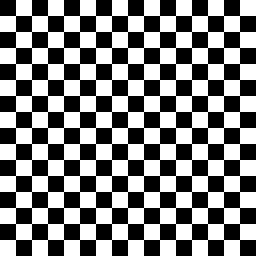
\includegraphics[width=1.25in]{figures/checker.jpg} 
\apiend

\vspace{10pt}
\begin{tinycode}
--pattern fill:top=0.1,0.1,0.1:bottom=0,0,0.5 640x480 3
--pattern fill:left=0.1,0.1,0.1:right=0,0.75,0 640x480 3
--pattern fill:topleft=.1,.1,.1:topright=1,0,0:bottomleft=0,1,0:botromright=0,0,1 640x480 3
\end{tinycode}

\noindent Horizontal, vertical, or 4-corner gradients.

\noindent \begin{tabular}{lll}

\includegraphics[width=1.5in]{figures/gradient.jpg} &
 
\includegraphics[width=1.5in]{figures/gradienth.jpg} &
 
\includegraphics[width=1.5in]{figures/gradient4.jpg}
\end{tabular}

\apiitem{\small oiiotool --pattern noise:type=uniform:min=1:max=1 256x256 3 -o colornoise.jpg \\
oiiotool --pattern noise:type=uniform:min=0:max=1:mono=1 256x256 3 -o greynoise.jpg}
\vspace{10pt}
The first example puts uniform noise independently in 3 channels, while the
second generates a single greyscale noise and replicates it in all channels.

\spc 
\includegraphics[width=1.25in]{figures/unifnoise3.jpg}
\spc 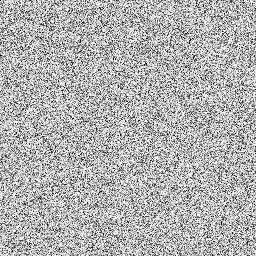
\includegraphics[width=1.25in]{figures/unifnoise1.jpg}
\apiend

\apiitem{\small oiiotool --pattern noise:type=gaussian:mean=0.5:stddev=0.2 256x256 3 -o gaussnoise.jpg}
\vspace{10pt}
Generate Gaussian noise with mean 0.5 and standard deviation 0.2 for each channel.

\spc 
\includegraphics[width=1.25in]{figures/gaussnoise.jpg}
\apiend

\apiend


\apiitem{\ce --kernel {\rm \emph{name size}}}
Create new 1-channel {\cf float} image big enough to hold the named
kernel and size (size is expressed as \emph{width}{\cf x}\emph{height},
e.g. {\cf 5x5}).  The \emph{width} and \emph{height} are allowed to be
floating-point numbers. The kernel image will have its origin offset so
that the kernel center is at (0,0), and and will be normalized (the sum
of all pixel values will be 1.0).

Kernel names can be: {\cf gaussian}, {\cf sharp-gaussian}, {\cf box},
{\cf triangle}, {\cf blackman-harris}, {\cf mitchell}, {\cf b-spline},
\qkw{cubic}, \qkw{keys}, \qkw{simon}, \qkw{rifman}, {\cf disk}.
There are also {\cf catmull-rom} and {\cf lanczos3}, but
they are fixed-size kernels that don't scale with the width, and are
therefore probably less useful in most cases.

\noindent Examples:

\begin{code}
    oiiotool --kernel gaussian 11x11 -o gaussian.exr
\end{code}
\apiend



\apiitem{\ce --capture}

Capture a frame from a camera device, pushing it onto the image stack
and making it the new current image.  Optional appended arguments
include:

\begin{tabular}{p{10pt} p{1in} p{3.5in}}
  & {\cf camera=}\emph{num} & Select which camera number to capture
  (default: 0).
\end{tabular}

\noindent Examples:

\begin{tabular}{p{2in} p{4in}}
    {\cf --capture}  &      Capture from the default camera. \\
    {\cf --capture:camera=1}  & Capture from camera \#1. \\
\end{tabular}
\apiend


\section{\oiiotool commands that do image processing}

\apiitem{{\ce --add} \\
{\ce --addc} {\rm \emph{value}} \\
{\ce --addc} {\rm \emph{value0,value1,value2...}}}

Replace the \emph{two} top images with a new image that is the pixel-by-
pixel sum of those images ({\cf --add}), or add a constant color value to
all pixels in the top image ({\cf --addc}).

For {\cf --addc}, if a single constant value is given, it will be added to
all color channels. Alternatively, a series of comma-separated constant
values (with no spaces!) may be used to specifiy a different value to add to
each channel in the image.

% \noindent Examples:

% \begin{tabular}{m{3in} m{2.5in}}
%   {\cf \footnotesize oiiotool tahoe.jpg --addc 0.5 -o addc.jpg}
%      & \includegraphics[width=1in]{figures/tahoe-small.jpg}
%          \raisebox{40pt}{\large $\rightarrow$}
%         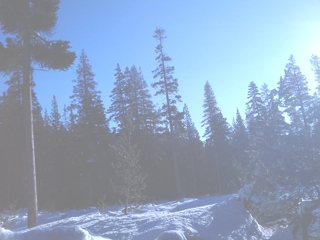
\includegraphics[width=1in]{figures/addc.jpg} \\
% \end{tabular}

\noindent Examples:
\begin{code}
    oiiotool tahoe.jpg --addc 0.5 -o addc.jpg
\end{code}
\spc \includegraphics[width=1.5in]{figures/tahoe-small.jpg}
\raisebox{40pt}{\large $\rightarrow$}
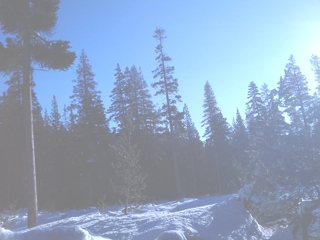
\includegraphics[width=1.5in]{figures/addc.jpg} \\

\vspace{12pt}

\begin{code}
    oiiotool imageA.tif imageB.tif --add -o sum.jpg
\end{code}
\apiend

\apiitem{{\ce --sub} \\
{\ce --subc} {\rm \emph{value}} \\
{\ce --subc} {\rm \emph{value0,value1,value2...}}}
Replace the \emph{two} top images with a new image that is the pixel-by-
pixel difference between the first and second images ({\cf --sub}), or
subtract a constant color value from all pixels in the top image ({\cf
--subc}).

For {\cf --subc}, if a single constant value is given, it will be subtracted
from all color channels. Alternatively, a series of comma-separated constant
values (with no spaces!) may be used to specifiy a different value to
subtract from each channel in the image.
\apiend

\apiitem{{\ce --mul} \\
{\ce --mulc} {\rm \emph{value}} \\
{\ce --mulc} {\rm \emph{value0,value1,value2...}}}
Replace the \emph{two} top images with a new image that is the pixel-by-
pixel multiplicative product of those images ({\cf --mul}), or multiply all
pixels in the top image by a constant value ({\cf --mulc}).

For {\cf --mulc}, if a single constant value is given, it will be multiplied
to all color channels. Alternatively, a series of comma-separated constant
values (with no spaces!) may be used to specifiy a different value to
multiply with each channel in the image.

\noindent Example:
\begin{code}
    oiiotool tahoe.jpg --mulc 0.2 -o mulc.jpg
\end{code}
\spc \includegraphics[width=1.5in]{figures/tahoe-small.jpg}
\raisebox{40pt}{\large $\rightarrow$}
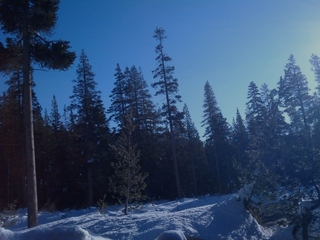
\includegraphics[width=1.5in]{figures/mulc.jpg} \\
\apiend

\apiitem{{\ce --div} \\
{\ce --divc} {\rm \emph{value}} \\
{\ce --divc} {\rm \emph{value0,value1,value2...}}}
Replace the \emph{two} top images with a new image that is the
pixel-by-pixel, channel-by-channel result of the first image divided by
the second image ({\cf --div}), or divide all
pixels in the top image by a constant value ({\cf --divc}).
Division by zero is defined as resulting in 0.

For {\cf --divc}, if a single constant value is given, all color channels
will have their values divided by the same value.  Alternatively, a series
of comma-separated constant values (with no spaces!) may be used to specifiy
a different multiplier for each channel in the image, respectively.
\apiend

\apiitem{{\ce --mad}}
Replace the \emph{three} top images A, B, and C (C being the top of stack, B
below it, and A below B), and compute A*B+C, placing the result on the
stack. Note that \qkw{A B C --mad} is equivalent to \qkw{A B --mul C --add},
though using {\cf --mad} may be somewhat faster and preserve more precision.

%\noindent Example:
%\begin{code}
%    oiiotool tahoe.jpg --mulc 0.2 -o mulc.jpg
%\end{code}
%\spc \includegraphics[width=1.5in]{figures/tahoe-small.jpg}
%\raisebox{40pt}{\large $\rightarrow$}
%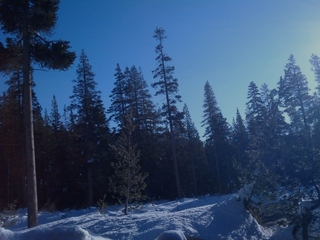
\includegraphics[width=1.5in]{figures/mulc.jpg} \\
\apiend


\apiitem{{\ce --invert}}
Replace the top images with its color inverse. It only inverts the first
three channels, in order to preserve alpha.

\noindent Example:
\begin{code}
   oiiotool tahoe.jpg --inverse -o inverse.jpg
\end{code}
\spc \includegraphics[width=1.5in]{figures/tahoe-small.jpg}
\raisebox{40pt}{\large $\rightarrow$}
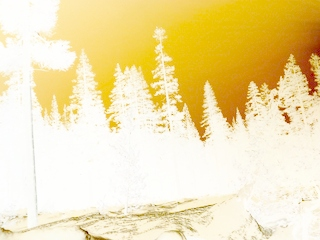
\includegraphics[width=1.5in]{figures/invert.jpg} \\
\apiend


\apiitem{{\ce --absdiff} \\
{\ce --absdiffc} {\rm \emph{value}} \\
{\ce --absdiffc} {\rm \emph{value0,value1,value2...}}}
Replace the \emph{two} top images with a new image that is the absolute
value of the difference between the first and second images ({\cf --absdiff}),
or replace the top image by the absolute value of the difference between each
pixel and a constant color ({\cf --absdiffc}).
\apiend

\apiitem{\ce --abs}
Replace the current image with a new image that has each pixel
consisting of the \emph{absolute value} of he old pixel value.
\apiend

\apiitem{\ce --powc {\rm \emph{value}} \\
--powc {\rm \emph{value0,value1,value2...}}}
Raise all the pixel values in the top image to a constant power value.
If a single constant value is given, all color channels will have their values
raised to this power.  Alternatively, a series of
comma-separated constant values (with no spaces!) may be used to specifiy a
different exponent for each channel in the image, respectively.
\apiend

\apiitem{\ce --noise}
Alter the top image to introduce noise, with the option {\cf :type=}
specifying the kind of noise: (1) {\cf gaussian} (default) for normal
distribution noise with mean and standard deviation given by {\cf :mean=}
and {\cf :stddev=}, respectively (defaulting to 0 and 0.1); (2) {\cf
uniform} for uniformly-distributed noise over the range of values given by
options {\cf :min=} and {\cf :max=} (defaults: 0 and 0.1); (3) {\cf salt}
for ``salt and pepper'' noise where a portion of pixels given by  option
{\cf portion=} (default: 0.1) is replaced with value given by option {\cf
value=} (default: 0).

For any of these noise types, the option {\cf seed=} can be used to change
the random number seed, {\cf mono=1} can be used to make monochromatic noise
(same value in all channels), and {\cf nchannels=} can be used to limit
which channels are affected by the noise

\noindent Example:
\begin{code}
    # Add color gaussian noise to an image
    oiiotool tahoe.jpg --noise:type=gaussian:stddev=0.1 -o noisy.jpg

    # Simulate bad pixels by turning 1% of pixels black, but only in RGB
    # channels (leave A alone)
    oiiotool tahoe-rgba.tif --noise:type=salt:value=0:portion=0.01:mono=1:nchannels=3 \
        -o dropouts.tif
\end{code}

\spc \begin{tabular}{lll}
\includegraphics[width=1.5in]{figures/tahoe-small.jpg} &
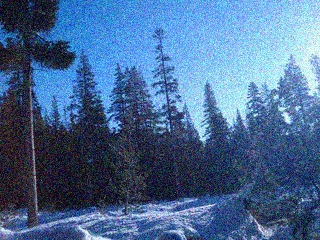
\includegraphics[width=1.5in]{figures/tahoe-gauss.jpg} &
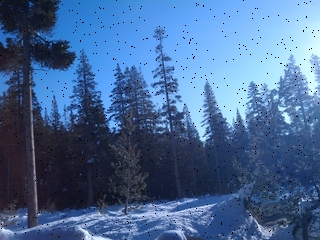
\includegraphics[width=1.5in]{figures/tahoe-pepper.jpg} \\
original & gaussian noise & salt \& pepper dropouts \\
\end{tabular}
\apiend

\apiitem{\ce --chsum}
Replaces the top image by a copy that contains only 1 color channel,
whose value at each pixel is the sum of all channels of the original
image.  Using the optional {\cf weight} allows you to customize the
weight of each channel in the sum.

\begin{tabular}{p{10pt} p{1in} p{3.5in}}
  & {\cf weight=}\emph{r,g,...} & Specify the weight of each channel
  (default: 1).
\end{tabular}

\noindent Example:
\begin{code}
    oiiotool RGB.tif --chsum:weight=.2126,.7152,.0722 -o luma.tif
\end{code}
\spc \includegraphics[width=1.5in]{figures/tahoe-small.jpg}
\raisebox{40pt}{\large $\rightarrow$}
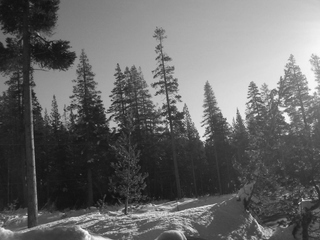
\includegraphics[width=1.5in]{figures/luma.jpg} \\
\apiend

\apiitem{\ce --contrast}
\NEW % 1.9
Remap pixel values from [black, white] to [min, max], with an optional
smooth sigmoidal contrast stretch as well.

Optional appended arguments include:

\begin{tabular}{p{10pt} p{1in} p{3.75in}}
 & {\cf black=}\emph{vals} & Specify black value(s), default 0.0. \\
 & {\cf white=}\emph{vals} & Specify white value(s), default 1.0. \\
 & {\cf min=}\emph{vals} & Specify the minimum range value(s), default 0.0. \\
 & {\cf max=}\emph{vals} & Specify the maximum range value(s), default 1.0. \\
 & {\cf scontrast=}\emph{vals} & Specify sigmoidal contrast slope value(s), default 1.0. \\
 & {\cf sthresh=}\emph{vals} & Specify sigmoidal threshold value(s) giving
        the position of maximum slope, default 0.5. \\
 & {\cf clamp=}\emph{on} & If \emph{on} is nonzero, will optionally clamp
                                    all result channels to [min,max].
\end{tabular}

\noindent Each \emph{vals} may be either a single floating point value
for all channels, or a comma-separated list of per-channel values.

\noindent Examples:
\begin{code}
    oiiotool tahoe.tif --contrast:black=0.1:white=0.75 -o linstretch.tif
    oiiotool tahoe.tif --contrast:black=1.0:white=0.0:clamp=0 -o inverse.tif
    oiiotool tahoe.tif --contrast:scontrast=5 -o sigmoid.tif
\end{code}

\noindent \begin{tabular}{cccc}
\includegraphics[width=1.1in]{figures/tahoe-small.jpg} &
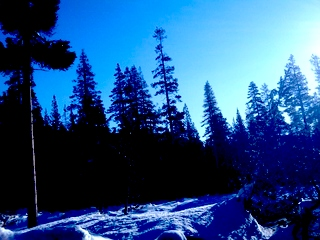
\includegraphics[width=1.1in]{figures/tahoe-lincontrast.jpg} &
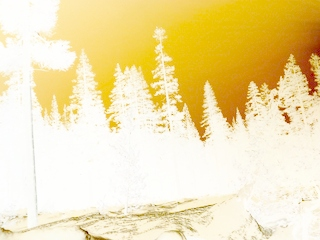
\includegraphics[width=1.1in]{figures/tahoe-inverse.jpg} &
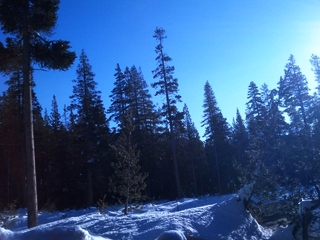
\includegraphics[width=1.1in]{figures/tahoe-sigmoid.jpg} \\
original & linstretch & inverse & sigmoid \\
\end{tabular}
\apiend


\apiitem{\ce --colormap {\rm \emph{mapname}}}
Creates an RGB color map based on the luminance of the input image. The
{\cf mapname} may be one of: \qkw{magma}, \qkw{inferno}, \qkw{plasma},
\qkw{viridis}, \qkw{blue-red}, \qkw{spectrum}, and \qkw{heat}.
Or, {\cf mapname} may also be a comma-separated list of RGB triples, to form
a custom color map curve.

\NEW % 1.9
Note that \qkw{magma}, \qkw{inferno}, \qkw{plasma}, \qkw{viridis} are
perceptually uniform, strictly increasing in luminance, look good when
converted to grayscale, and work for people with all types of
colorblindness. These are all desirable qualities that are lacking in the
other, older, crappier maps (blue-red, spectrum, and heat). Don't be fooled
by the flashy \qkw{spectrum} colors --- it is an empirically bad color map
compared to the preferred ones.

\noindent Example:
\begin{code}
    oiiotool tahoe.jpg --colormap inferno -o inferno.jpg
    oiiotool tahoe.jpg --colormap viridis -o viridis.jpg
    oiiotool tahoe.jpg --colormap spectrum -o spectrum.jpg
    oiiotool tahoe.jpg --colormap .25,.25,.25,0,.5,0,1,0,0 -o custom.jpg
\end{code}

\noindent \begin{tabular}{lllll}
\includegraphics[width=0.9in]{figures/tahoe-small.jpg} &
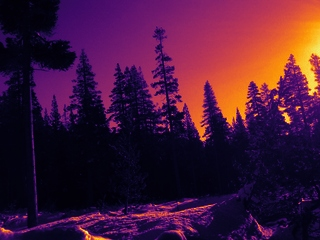
\includegraphics[width=0.9in]{figures/colormap-inferno.jpg} &
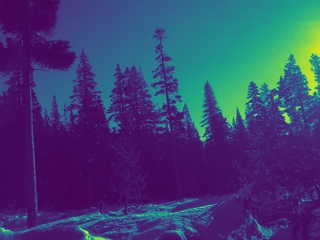
\includegraphics[width=0.9in]{figures/colormap-viridis.jpg} &
\includegraphics[width=0.9in]{figures/colormap-spectrum.jpg} &
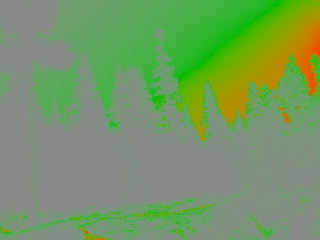
\includegraphics[width=0.9in]{figures/colormap-custom.jpg} \\
original & inferno & viridis & spectrum & custom values \\
\end{tabular}
\apiend


\apiitem{\ce --paste {\rm \emph{location}}}
Takes two images -- the first is the ``foreground'' and the second is
the ``background'' -- and uses the pixels of the foreground to replace
those of the backgroud beginning at the upper left \emph{location}
(expressed as {\cf +}\emph{xpos}{\cf +}\emph{ypos}, e.g., {\cf +100+50},
or of course using {\cf -} for negative offsets).
\apiend

\apiitem{\ce --mosaic {\rm \emph{size}}}
Removes \emph{w}{\cf x}\emph{h} images, dictated by the
\emph{size}, and turns them into a single image mosaic.
Optional appended arguments
include:

\begin{tabular}{p{10pt} p{1in} p{3.5in}}
  & {\cf pad=}\emph{num} & Select the number of pixels of black padding
    to add between images (default: 0).
\end{tabular}

\noindent Examples:
\begin{code}
    oiiotool left.tif right.tif --mosaic:pad=16 2x1 -o out.tif

    oiiotool 0.tif 1.tif 2.tif 3.tif 4.tif --mosaic:pad=16 2x2 -o out.tif
\end{code}
\apiend

\apiitem{\ce --over}
\index{composite}
Replace the \emph{two} top images with a new image that is the
Porter/Duff ``over'' composite with the first image as the foreground
and the second image as the background.
Both input images must have the same number and order of channels
and must contain an alpha channel.
\apiend

\apiitem{\ce --zover}
\index{depth composite}
Replace the \emph{two} top images with a new image that is a \emph{depth
composite} of the two images -- the operation is the 
Porter/Duff ``over'' composite, but each pixel individually will choose
which of the two images is the foreground and which background, depending on
the ``Z'' channel values for that pixel (larger Z means farther away).
Both input images must have the same number and order of channels
and must contain both depth/Z and alpha channels. Optional appended arguments
include:

\begin{tabular}{p{10pt} p{1in} p{3.5in}}
  & {\cf zeroisinf=}\emph{num} & If nonzero, indicates that $z=0$ pixels
  should be treated as if they were infinitely far away. (The default is
  0, meaning that ``zero means zero.'').
\end{tabular}

\apiend

\apiitem{\ce --rotate90}
Replace the current image with a new image that is rotated 90 degrees
clockwise.

\noindent Example:
\begin{code}
    oiiotool grid.jpg --rotate90 -o rotate90.jpg
\end{code}
\spc \includegraphics[width=1.25in]{figures/grid-small.jpg}
\raisebox{40pt}{\large $\rightarrow$}
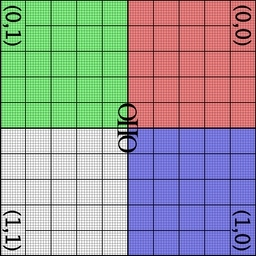
\includegraphics[width=1.25in]{figures/rotate90.jpg} \\
\apiend

\apiitem{\ce --rotate180}
Replace the current image with a new image that is rotated by
180 degrees.

\noindent Example:
\begin{code}
    oiiotool grid.jpg --rotate180 -o rotate180.jpg
\end{code}
\spc \includegraphics[width=1.25in]{figures/grid-small.jpg} 
\raisebox{40pt}{\large $\rightarrow$}
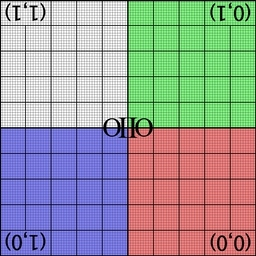
\includegraphics[width=1.25in]{figures/rotate180.jpg} \\
\apiend

\apiitem{\ce --rotate270}
Replace the current image with a new image that is rotated 270 degrees
clockwise (or 90 degrees counter-clockwise).

\noindent Example:
\begin{code}
    oiiotool grid.jpg --rotate270 -o rotate270.jpg
\end{code}
\spc \includegraphics[width=1.25in]{figures/grid-small.jpg}
\raisebox{40pt}{\large $\rightarrow$}
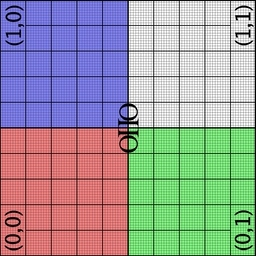
\includegraphics[width=1.25in]{figures/rotate270.jpg} \\
\apiend

\apiitem{\ce --flip}
Replace the current image with a new image that is flipped vertically,
with the top scanline becoming the bottom, and vice versa.

\noindent Example:
\begin{code}
    oiiotool grid.jpg --flip -o flip.jpg
\end{code}
\spc \includegraphics[width=1.25in]{figures/grid-small.jpg} 
\raisebox{40pt}{\large $\rightarrow$}
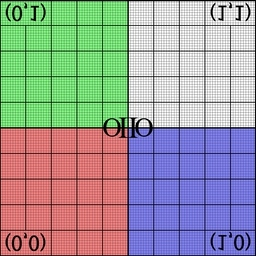
\includegraphics[width=1.25in]{figures/flip.jpg} \\
\apiend

\apiitem{\ce --flop}
Replace the current image with a new image that is flopped horizontally,
with the leftmost column becoming the rightmost, and vice versa.

\noindent Example:
\begin{code}
    oiiotool grid.jpg --flop -o flop.jpg
\end{code}
\spc \includegraphics[width=1.25in]{figures/grid-small.jpg} 
\raisebox{40pt}{\large $\rightarrow$}
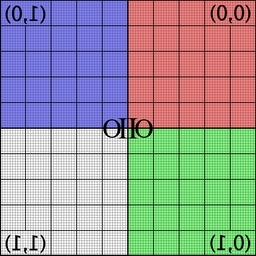
\includegraphics[width=1.25in]{figures/flop.jpg} \\
\apiend

\apiitem{\ce --reorient}
Replace the current image with a new image that is rotated and/or flipped
as necessary to move the pixels to match the Orientation metadata
that describes the desired display orientation.

\noindent Example:
\begin{code}
    oiiotool tahoe.jpg --reorient -o oriented.jpg
\end{code}
%\spc \includegraphics[width=1.25in]{figures/grid-small.jpg} 
%\raisebox{40pt}{\large $\rightarrow$}
%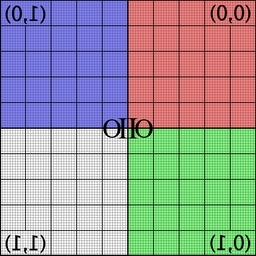
\includegraphics[width=1.25in]{figures/flop.jpg} \\
\apiend

\apiitem{\ce --transpose}
Replace the current image with a new image that is trasposed about
the $xy$ axis (x and coordinates and size are flipped).

\noindent Example:
\begin{code}
    oiiotool grid.jpg --transpose -o transpose.jpg
\end{code}
\spc \includegraphics[width=1.25in]{figures/grid-small.jpg} 
\raisebox{40pt}{\large $\rightarrow$}
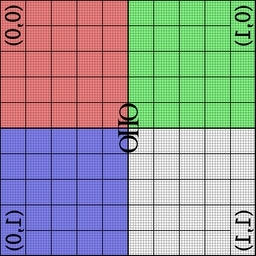
\includegraphics[width=1.25in]{figures/transpose.jpg} \\
\apiend

\apiitem{\ce --cshift {\rm \emph{offset}}}
Circularly shift the pixels of the image by the given offset (expressed
as {\cf +10+100} to move by 10 pixels horizontally and 100 pixels
vertically, or {\cf +50-30} to move by 50 pixels horizontally and
$-30$ pixels vertically.  \emph{Circular} shifting means that the
pixels wrap to the other side as they shift.

\noindent Example:
\begin{code}
    oiiotool grid.jpg --cshift +70+30 -o cshift.jpg
\end{code}
\spc \includegraphics[width=1.25in]{figures/grid-small.jpg} 
\raisebox{40pt}{\large $\rightarrow$}
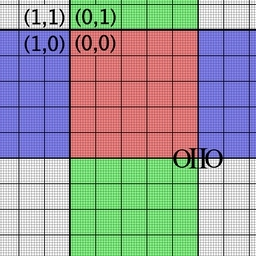
\includegraphics[width=1.25in]{figures/cshift.jpg} \\
\apiend

\apiitem{\ce --crop {\rm \emph{size}}}
Replace the current image with a new copy with the given \emph{size},
cropping old pixels no longer needed, padding black pixels where they
previously did not exist in the old image, and adjusting the offsets
if requested.

The size is in the form 
\\ \spc\spc \emph{width}\,{\cf x}\,\emph{height}{\cf [+-]}\emph{xoffset}{\cf
  [+-]}\emph{yoffset}
\\ or~~~~ \spc \emph{xmin,ymin,xmax,ymax} \\


Note that {\cf crop} does not \emph{reposition} pixels, it only trims or
pads to reset the image's pixel data window to the specified region.

If \oiiotool's global {\cf -a} flag is used ({\bf a}ll subimages)), or if the
optional {\cf --crop:allsubimages=1} is employed, the crop will be applied
identically to all subimages.

\noindent Examples:

\begin{code}
    # Both of these crop to a 100x120 region that begins at x=35,y=40
    oiiotool tahoe.exr --crop 100x120+35+40 -o crop.exr
    oiiotool tahoe.exr --crop 35,40,134,159 -o crop.exr
\end{code}

\hspace{0.4in} \includegraphics[width=1.5in]{figures/tahoe-small.jpg}
\raisebox{40pt}{\large $\rightarrow$}
 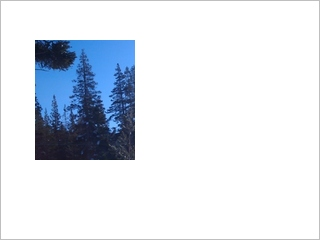
\includegraphics[width=1.5in]{figures/crop.jpg}
\apiend

\apiitem{\ce --croptofull}
Replace the current image with a new image that is cropped or padded
as necessary to make the pixel data window exactly cover
the full/display window.
\apiend

\apiitem{\ce --trim}
Replace the current image with a new image that is cropped to contain the
minimal rectangular ROI that contains all of the nonzero-valued pixels of
the original image.

\noindent Examples:

\begin{code}
    oiiotool greenrect.exr -trim -o trimmed.jpg
\end{code}
\hspace{0.4in} 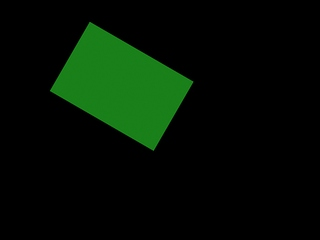
\includegraphics[width=1.5in]{figures/pretrim.jpg}
\raisebox{40pt}{\large $\rightarrow$}
 \includegraphics[width=1.5in]{figures/trim.jpg}
\apiend

\apiitem{\ce --cut {\rm \emph{size}}}
Replace the current image with a new copy with the given \emph{size},
cropping old pixels no longer needed, padding black pixels where they
previously did not exist in the old image, repositioning the cut region
at the image origin (0,0) and resetting the full/display window to be
identical to the new pixel data window.  (In other words, {\cf --cut}
is equavalent to {\cf --crop} followed by {\cf --origin +0+0 --fullpixels}.)

The size is in the form 
\\ \spc\spc \emph{width}\,{\cf x}\,\emph{height}{\cf [+-]}\emph{xoffset}{\cf
  [+-]}\emph{yoffset}
\\ or~~~~ \spc \emph{xmin,ymin,xmax,ymax} \\

\noindent Examples:

\begin{code}
    # Both of these crop to a 100x120 region that begins at x=35,y=40
    oiiotool tahoe.exr --cut 100x120+35+40 -o cut.exr
    oiiotool tahoe.exr --cut 35,40,134,159 -o cut.exr
\end{code}

\hspace{0.4in} \includegraphics[width=1.5in]{figures/tahoe-small.jpg}
\raisebox{40pt}{\large $\rightarrow$}
\raisebox{0.55in}{\includegraphics[width=0.476in]{figures/cut.jpg}}
\apiend

\apiitem{\ce --resample {\rm \emph{size}}}
Replace the current image with a new image that is resampled to the
given pixel data resolution rapidly, but at a low quality, either by simple
bilinear interpolation or by just
copying the ``closest'' pixel.  The \emph{size} is in the form
\\ \spc\spc \emph{width}\,{\cf x}\,\emph{height}{\cf [+-]}\emph{xoffset}{\cf
  [+-]}\emph{yoffset}
\\ or~~~~ \spc \emph{xmin,ymin,xmax,ymax} \\
\\ or~~~~ \spc \emph{scale}{\verb|%|} \\
\\ or~~~~ \spc \emph{wscale}{\verb|%|}\,{\cf x}\,\emph{hscale}{\verb|%|} \\

\noindent if {\cf width} or {\cf height} is 0, that dimension will be
automatically computed so as to preserve the original aspect ratio.

Optional appended arguments include:

\begin{tabular}{p{10pt} p{1in} p{3.75in}}
 & {\cf interp=}\emph{bool} & If set to zero, it will just copy the
 ``closest'' pixel; if nonzero, bilinear interpolation of the surrounding
 4 pixels will be used. \\
\end{tabular}


\noindent Examples (suppose that the original image is 640x480):

\begin{tabular}{p{2in} p{4in}}
    {\cf --resample 1024x768}  &     new resolution w=1024, h=768 \\
    {\cf --resample 50{\verb|%|}}  & reduce resolution to 320x240 \\
    {\cf --resample 300{\verb|%|}}  & increase resolution to 1920x1440 \\
    {\cf --resample 400x0}  &     new resolution will be 400x300
\end{tabular}

\apiend

\apiitem{\ce --resize {\rm \emph{size}}}
Replace the current image with a new image whose display (full) size is
the given pixel data resolution and offset.  The \emph{size} is in the form 
\\ \spc\spc \emph{width}\,{\cf x}\,\emph{height}{\cf [+-]}\emph{xoffset}{\cf
  [+-]}\emph{yoffset}
\\ or~~~~ \spc \emph{xmin,ymin,xmax,ymax} \\
\\ or~~~~ \spc \emph{scale}{\verb|%|} \\
\\ or~~~~ \spc \emph{wscale}{\verb|%|}\,{\cf x}\,\emph{hscale}{\verb|%|} \\

\noindent if {\cf width} or {\cf height} is 0, that dimension will be
automatically computed so as to preserve the original aspect ratio.

Optional appended arguments include:

\begin{tabular}{p{10pt} p{1in} p{3.75in}}
 & {\cf filter=}\emph{name} & Filter name. The default is {\cf
  blackman-harris} when increasing resolution, {\cf lanczos3} when
decreasing resolution. \\
\end{tabular}

\noindent Examples (suppose that the original image is 640x480):

\begin{tabular}{p{2in} p{4in}}
    {\cf --resize 1024x768}  &     new resolution w=1024, h=768 \\
    {\cf --resize 50{\verb|%|}}  & reduce resolution to 320x240 \\
    {\cf --resize 300{\verb|%|}}  & increase resolution to 1920x1440 \\
    {\cf --resize 400x0}  &     new resolution will be 400x300
\end{tabular}

\apiend

\apiitem{\ce --fit {\rm \emph{size}}}
Replace the current image with a new image that is resized to fit
into the given pixel data resolution, keeping the original aspect ratio
and padding with black pixels if the requested image size does not
have the same aspect ratio.  The \emph{size} is in the form 
\\ \spc\spc \emph{width}\,{\cf x}\,\emph{height}
\\ or~~~~ \spc \emph{width}\,{\cf x}\,\emph{height}{\cf [+-]}\emph{xorigin}{\cf [+-]}\emph{yorigin} \\

Optional appended arguments include:

\begin{tabular}{p{10pt} p{1in} p{3.75in}}
 & {\cf filter=}\emph{name} & Filter name. The default is {\cf
  blackman-harris} when increasing resolution, {\cf lanczos3} when
decreasing resolution. \\
 & {\cf pad=}\emph{p} & If the argument is nonzero, will pad with
  black pixels to make the resulting image exactly the size specified, if
  the source and desired size are not the same aspect ratio. \\
 & {\cf exact=}\emph{e} & If the argument is nonzero, will result in an
  exact match on aspect ratio and centering (partial pixel shift if necessary),
  whereas the default (0) will only preserve aspect ratio and centering
  to the precision of a whole pixel. \\
 & {\cf wrap=}\emph{w} & For ``exact'' aspect ratio fitting, this determines
  the wrap mode used for the resizing kernel (default: \qkw{black}, other
  choices include \qkw{clamp}, \qkw{periodic}, \qkw{mirror}).
\end{tabular}

\noindent Examples:

\begin{code}
    oiiotool in.exr --fit:pad=1:exact=1 640x480 -o out.exr

    oiiotool in.exr --fit 1024x1024 -o out.exr
\end{code}
\apiend

\apiitem{\ce --pixelaspect {\rm \emph{aspect}}}
Replace the current image with a new image that scales up the width or
height in order to match the requested pixel aspect ratio.  If displayed
in a manner that honors the PixelAspectRatio, it should look the same,
but it will have different pixel dimensions than the original. It will
always be the same or higher resolution, so it does not lose any detail
present in the original.

As an example, if you have a $512 \times 512$ image with pixel aspect
ratio 1.0, {\cf --pixelaspect 2.0} will result in a $512 \times 1024$
image that has \qkw{PixelAspectRatio} metadata set to 2.0.

Optional appended arguments include:

\begin{tabular}{p{10pt} p{1.25in} p{3.5in}}
 & {\cf filter=}\emph{name} & Filter name. The default is \qkw{lanczos3}. \\
\end{tabular}

\noindent Examples:

\begin{tinycode}
  oiiotool mandrill.tif --pixelaspect 2.0 -o widepixels.tif
\end{tinycode}
%\spc \includegraphics[width=1.25in]{figures/grid-small.jpg}
%\raisebox{40pt}{\large $\rightarrow$}
%\includegraphics[width=1.25in]{figures/rotate45.jpg} \\
\apiend


\apiitem{\ce --rotate {\rm \emph{angle}}}
Replace the current image with a new image that is rotated by the given
angle (in degrees). Positive angles mean to rotate counter-clockwise,
negative angles mean clockwise. By default, the center of rotation is at the
exact center of the display window (a.k.a.\ ``full'' image), but can be
explicitly set with the optional {\cf center=\emph{x,y}} option.

Optional appended arguments include:

\begin{tabular}{p{10pt} p{1.25in} p{3.5in}}
 & {\cf center=}\emph{x,y} & Alternate center of rotation. \\
 & {\cf filter=}\emph{name} & Filter name. The default is \qkw{lanczos3}. \\
 & {\small \cf recompute_roi=}\emph{val} & If nonzero, recompute the pixel data
     window to exactly hold the transformed image (default=0). \\
\end{tabular}

\noindent Examples:

\begin{tinycode}
  oiiotool mandrill.tif --rotate 45 -o rotated.tif

  oiiotool mandrill.tif --rotate:center=80,91.5:filter=lanczos3 45 -o rotated.tif
\end{tinycode}
\spc \includegraphics[width=1.25in]{figures/grid-small.jpg} 
\raisebox{40pt}{\large $\rightarrow$}
\includegraphics[width=1.25in]{figures/rotate45.jpg} \\
\apiend


\apiitem{\ce --warp {\rm \emph{M33}}}
Replace the current image with a new image that is warped by the given
$3 \times 3$ matrix (presented as a comma-separated list of values, without
any spaces).

Optional appended arguments include:

\begin{tabular}{p{10pt} p{1.25in} p{3.5in}}
 & {\cf filter=}\emph{name} & Filter name. The default is \qkw{lanczos3}. \\
 & {\small\cf recompute_roi=}\emph{val} & If nonzero, recompute the pixel data
     window to exactly hold the transformed image (default=0). \\
\end{tabular}

\noindent Examples:

\begin{tinycode}
  oiiotool mandrill.tif --warp "0.707,0.707,0,-0.707,0.707,0,128,-53.02,1" -o warped.tif
\end{tinycode}
\apiend


\apiitem{\ce --convolve}
Use the top image as a kernel to convolve the next image farther down
the stack, replacing both with the result.

\noindent Examples:
\begin{code}
    # Use a kernel image already prepared
    oiiotool image.exr kernel.exr --convolve -o output.exr

    # Construct a kernel image on the fly with --kernel
    oiiotool image.exr --kernel gaussian 5x5 --convolve -o blurred.exr
\end{code}
\apiend

\apiitem{\ce --blur {\rm \emph{size}}}
Blur the top image with a blur kernel of the given size expressed as
\emph{width}{\cf x}\emph{height}.  (The sizes may be floating point 
numbers.)

Optional appended arguments include:

\begin{tabular}{p{10pt} p{1in} p{3.75in}}
 & {\cf kernel=}\emph{name} & Kernel name. The default is {\cf gaussian}.
\end{tabular}

\noindent Examples:
\begin{code}
    oiiotool image.jpg --blur 5x5 -o blurred.jpg

    oiiotool image.jpg --blur:kernel=bspline 7x7 -o blurred.jpg
\end{code}

\spc \begin{tabular}{ll}
\includegraphics[width=1.5in]{figures/tahoe-small.jpg} &
\includegraphics[width=1.5in]{figures/tahoe-blur.jpg} \\
original & blurred \\
\end{tabular}
\apiend


\apiitem{\ce --median {\rm \emph{size}}}
Perform a median filter on the top image with a window of the given size
expressed as \emph{width}{\cf x}\emph{height}.  (The sizes are integers.)
This helps to eliminate noise and other unwanted high-frequency detail, but
without blurring long edges the way a {\cf --blur} command would.

\noindent Examples:
\begin{code}
    oiiotool noisy.jpg --median 3x3 -o smoothed.jpg
\end{code}

\spc \begin{tabular}{lll}
\includegraphics[width=1.5in]{figures/tahoe-small.jpg} &
\includegraphics[width=1.5in]{figures/tahoe-pepper.jpg} &
\includegraphics[width=1.5in]{figures/tahoe-pepper-median.jpg} \\
original & with dropouts & median filtered \\
\end{tabular}
\apiend


\apiitem{\ce --dilate {\rm \emph{size}}\\
\ce --erode {\rm \emph{size}}}
\indexapi{dilate} \indexapi{erode}
\index{morphological filtering}

Perform dilation or erosion on the top image with a window of the given size
expressed as \emph{width}{\cf x}\emph{height}. (The sizes are integers.)
Dilation takes the maximum of pixel values inside the window, and makes
bright features wider and more prominent, dark features thinner, and removes
small isolated dark spots. Erosion takes the minimum of pixel values inside
the window, and makes dark features wider, bright features thinner, and
removes small isolated bright spots.

\noindent Examples:
\begin{code}
    oiiotool orig.tif --dilate 3x3 -o dilate.tif
    oiiotool orig.tif --erode 3x3 -o erode.tif
    oiiotool orig.tif --erode 3x3 --dilate 3x3 -o open.tif
    oiiotool orig.tif --dilate 3x3 --erode 3x3 -o close.tif
    oiiotool orig.tif --dilate 3x3 --erode 3x3 -sub -o gradient.tif
    oiiotool orig.tif open.tif -o tophat.tif
    oiiotool close.tif orig.tif -o bottomhat.tif
\end{code}

\spc \begin{tabular}{llll}
\includegraphics[width=0.75in]{figures/morphsource.jpg} &
\includegraphics[width=0.75in]{figures/dilate.jpg} &
\includegraphics[width=0.75in]{figures/erode.jpg} &
\includegraphics[width=0.75in]{figures/morphopen.jpg} \\
original & dilate & erode & open \\
\includegraphics[width=0.75in]{figures/morphclose.jpg} &
\includegraphics[width=0.75in]{figures/morphgradient.jpg} &
\includegraphics[width=0.75in]{figures/tophat.jpg} &
\includegraphics[width=0.75in]{figures/bottomhat.jpg} \\
close & gradient & tophat & bottomhat \\
\end{tabular}

\apiend


\apiitem{\ce --laplacian}
Calculates the Laplacian of the top image.

\noindent Examples:
\begin{code}
    oiiotool tahoe.jpg --laplacian tahoe-laplacian.exr
\end{code}

\spc \begin{tabular}{ll}
\includegraphics[width=1.5in]{figures/tahoe-small.jpg} &
\includegraphics[width=1.5in]{figures/tahoe-laplacian.jpg} \\
original & Laplacian image \\
\end{tabular}
\apiend


\apiitem{\ce --unsharp}
Unblur the top image using an ``unsharp mask.'' 

Optional appended arguments include:

\begin{tabular}{p{10pt} p{1in} p{3.75in}}
 & {\cf kernel=}\emph{name} & Name of the blur kernel (default: {\cf
    gaussian}). If the kernel name is {\cf median}, the unsarp mask
    algorithm will use a median filter rather than a blurring filter
    in order to compute the low-frequency image. \\
 & {\cf width=}\emph{w} & Width of the blur kernel (default: 3). \\
 & {\cf contrast=}\emph{c} & Contrast scale (default: 1.0) \\
 & {\cf threshold=}\emph{t} & Threshold for applying the difference
  (default: 0)
\end{tabular}

\noindent Examples:
\begin{code}
    oiiotool image.jpg --unsharp -o sharper.jpg

    oiiotool image.jpg --unsharp:width=5:contrast=1.5 -o sharper.jpg

    oiiotool image.jpg --unsharp:kernel=median -o sharper.jpg
    # Note: median filter helps emphasize compact high-frequency details
    # without over-sharpening long edges as the default unsharp filter
    # sometimes does.
\end{code}
% FIXME - should have a visual example
\apiend


\apiitem{\ce --fft \\
--ifft}
Performs forward and inverse unitized discrete Fourier transform.
The forward FFT always transforms only the first channel of the
top image on the stack, and results in a 2-channel image (with real and
imaginary channels).  The inverse FFT transforms the first two
channels of the top image on the stack (assuming they are real and
imaginary, respectively) and results in a single channel result (with
the real component only of the spatial domain result).

\noindent Examples:
\begin{code}
    # Select the blue channel and take its DCT
    oiiotool image.jpg --ch 2 --fft -o fft.exr

    # Reconstruct from the FFT
    oiiotool fft.exr --ifft -o reconstructed.exr

    # Output the power spectrum: real^2 + imag^2
    oiiotool fft.exr --dup --mul --chsum -o powerspectrum.exr
\end{code}
\apiend


\apiitem{\ce --polar \\
--unpolar}
The {\cf --polar} transforms a 2-channel image whose channels are
interpreted as complex values (real and imaginary components) into the
equivalent values expressed in polar form of amplitude and phase (with phase
between $0$ and $2\pi$).

The {\cf unpolar} performs the reverse transformation, converting from 
polar values (amplitude and phase) to complex (real and imaginary).

\noindent Examples:
\begin{code}
    oiiotool complex.exr --polar -o polar.exr
    oiiotool polar.exr --unpolar -o complex.exr
\end{code}
\apiend


\apiitem{\ce --fixnan {\rm \emph{streategy}}}
Replace the top image with a copy in which any pixels that contained
{\cf NaN} or {\cf Inf} values (hereafter referred to collectively as
``nonfinite'') are repaired.  If \emph{strategy} is {\cf black},
nonfinite values will be replaced with {\cf 0}.  If \emph{strategy} is
{\cf box3}, nonfinite values will be replaced by the average of all the
finite values within a $3 \times 3$ region surrounding the pixel.
If \emph{strategy} is
{\cf error}, nonfinite values will be left alone, but it will result in an
error that will terminate \oiiotool.
\apiend

\apiitem{\ce --clamp}
Replace the top image with a copy in which pixel values have been
clamped.  Optional arguments include:

Optional appended arguments include:

\begin{tabular}{p{10pt} p{1in} p{3.75in}}
 & {\cf min=}\emph{val} & Specify a minimum value for all channels. \\
 & {\cf min=}\emph{val0,val1,...} & Specify minimum value for each 
                                    channel individually. \\
 & {\cf max=}\emph{val} & Specify a maximum value for all channels. \\
 & {\cf max=}\emph{val0,val1,...} & Specify maximum value for each 
                                    channel individually. \\
 & {\cf clampalpha=}\emph{val} & If \emph{val} is nonzero, will 
                                    additionally clamp the alpha channel
                                    to [0,1].  (Default: 0, no
                                    additional alpha clamp.)
\end{tabular}

If no value is given for either the minimum or maximum, it will NOT
clamp in that direction.  For the variety of minimum and maximum that
specify per-channel values, a missing value indicates that the
corresponding channel should not be clamped.  

\noindent Examples:

\begin{tabular}{p{2in} p{4in}}
    {\cf --clamp:min=0} & Clamp all channels to a mimimum of 0 (all \\
                        &  negative values are changed to 0). \\
    {\cf --clamp:min=0:max=1} & Clamp all channels to [0,1]. \\
    {\cf --clamp:clampalpha=1} & Clamp the designated alpha channel to [0,1]. \\
    {\cf --clamp:min=,,0:max=,,3.0} & Clamp the third channel to [0,3],
                                      do not clamp \\ & other channels.
\end{tabular}

\apiend

\apiitem{\ce --rangecompress \\
--rangeexpand}
Range compression re-maps input values to a logarithmic scale.
Range expansion is the inverse mapping back to a linear scale.
Range compression and expansion only applies to color
channels; alpha or z channels will not be modified.

By default, this transformation will happen to each color channel 
independently.  But if the optional {\cf luma} argument is nonzero and
the image has at least 3 channels and the first three channels are
not alpha or depth, they will be assumed to be RGB and the pixel scaling
will be done using the luminance and applied equally to all color
channels. This can help to preserve color even when remapping intensity.

Optional appended arguments include:

\begin{tabular}{p{10pt} p{1in} p{3.75in}}
 & {\cf luma=}\emph{val} & If \emph{val} is 0, turns off the luma behavior.
\end{tabular}

Range compression and expansion can be useful in cases where high
contrast super-white ($> 1$) pixels (such as very bright highlights in
HDR captured or rendered images) can produce undesirable artifacts, such
as if you resize an HDR image using a filter with negative lobes --
which could result in objectionable ringing or even negative result
pixel values.  For example,

\begin{smallcode}
    oiiotool hdr.exr --rangecompress --resize 512x512 --rangeexpand -o resized.exr
\end{smallcode}
\apiend

\apiitem{\ce --fillholes}
Replace the top image with a copy in which any pixels that had
$\alpha < 1$ are ``filled'' in a smooth way using data from
surrounding $\alpha > 0$ pixels, resulting in an image that is
$\alpha = 1$ and plausible color everywhere.
This can be used both to fill internal ``holes'' as well as to extend an
image out.
\apiend


\apiitem{\ce --line {\rm \emph{x1,y1,x2,y2,...}}}
Draw (rasterize) an open polyline connecting the list of pixel positions, as
a comma-separated list of alternating $x$ and $y$ values. Additional
optional arguments include:

\begin{tabular}{p{10pt} p{1in} p{3.75in}}
 & {\cf color=}\emph{r,g,b,...} & specify the color of the line \\
\end{tabular}

The default color, if not supplied, is opaque white.

\noindent Examples:

\begin{code}
    oiiotool checker.exr --line:color=1,0,0 10,60,250,20,100,190 -o out.exr
\end{code}
\spc \includegraphics[width=2in]{figures/lines.png}  \\
\apiend


\apiitem{\ce --box {\rm \emph{x1,y1,x2,y2}}}
Draw (rasterize) a filled or unfilled a box with opposite corners {\cf (x1,y1)}
and {\cf (x2,y2)}. Additional optional arguments include:

\begin{tabular}{p{10pt} p{1in} p{3.75in}}
 & {\cf color=}\emph{r,g,b,...} & specify the color of the lines \\
 & {\cf fill=}\emph{bool} & if nonzero, fill in the box \\
\end{tabular}

The default color, if not supplied, is opaque white.

\noindent Examples:

\begin{code}
    oiiotool checker.exr --box:color=0,1,1,1 150,100,240,180 \
                 --box:color=0.5,0.5,0,0.5:fill=1 100,50,180,140 -o out.exr
\end{code}
\spc \includegraphics[width=2in]{figures/box.png}  \\
\apiend


\apiitem{\ce --fill {\rm \emph{size}}}
Alter the top image by filling the ROI specified by \emph{size}.
The fill can be a constant color, vertical gradient, horizontal gradient,
or four-corner gradient.

Optional arguments for constant color: \\
\begin{tabular}{p{10pt} p{1.5in} p{3.75in}}
 & {\cf color=}\emph{r,g,b,...} & the color of the constant \\
\end{tabular}

Optional arguments for vertical gradient: \\
\begin{tabular}{p{10pt} p{1.5in} p{3.75in}}
 & {\cf top=}\emph{r,g,b,...}    & the color for the top edge of the region \\
 & {\cf bottom=}\emph{r,g,b,...} & the color for the bottom edge of the region \\
\end{tabular}

Optional arguments for horizontal gradient: \\
\begin{tabular}{p{10pt} p{1.5in} p{3.75in}}
 & {\cf left=}\emph{r,g,b,...}  & the color for the left edge of the region \\
 & {\cf right=}\emph{r,g,b,...} & the color for the right edge of the region \\
\end{tabular}

Optional arguments for 4-corner gradient: \\
\begin{tabular}{p{10pt} p{1.5in} p{3.75in}}
 & {\cf topleft=}\emph{r,g,b,...}     & the color for the top left corner of the region \\
 & {\cf topright=}\emph{r,g,b,...}    & the color for the top right corner of the region \\
 & {\cf bottomleft=}\emph{r,g,b,...}  & the color for the bottom left corner of the region \\
 & {\cf bottomright=}\emph{r,g,b,...} & the color for the bottom right corner of the region \\
\end{tabular}


\noindent Examples:

\begin{smallcode}
    # make a grey-to-blue vertical gradient
    oiiotool --create 640x480 3 \
        --fill:top=0.1,0.1,0.1:bottom=0,0,0.5 640x480 -o gradient.tif

    # make a grey-to-green horizontal gradient
    oiiotool --create 640x480 3 \
        --fill:left=0.1,0.1,0.1:right=0,0.75,0 640x480 -o gradient.tif
\end{smallcode}
\begin{tinycode}
    # four-corner interpolated gradient
    oiiotool --create 640x480 3 \
        -fill:topleft=.1,.1,.1:topright=1,0,0:bottomleft=0,1,0:botromright=0,0,1 \
            640x480 -o gradient.tif
\end{tinycode}
\noindent \begin{tabular}{lll}
\includegraphics[width=1.5in]{figures/gradient.jpg} &
 \includegraphics[width=1.5in]{figures/gradienth.jpg} &
 \includegraphics[width=1.5in]{figures/gradient4.jpg}
\end{tabular}

\apiend


\apiitem{\ce --text {\rm \emph{words}}}
Draw (rasterize) text overtop of the current image.

\begin{tabular}{p{10pt} p{1in} p{3.75in}}
 & {\cf x=}\emph{xpos} & $x$ position (in pixel coordinates) of the text \\
 & {\cf y=}\emph{ypos} & $y$ position (in pixel coordinates) of the text  \\
 & {\cf size=}\emph{size} & font size (height, in pixels) \\
 & {\cf font=}\emph{name} & font name, full path to the font file on
  disk (use double quotes {\cf "name"} if the path name includes spaces) \\
 & {\cf color=}\emph{r,g,b,...} & specify the color of the text \\
 & {\cf xalign=}\emph{val} & controls horizontal text alignment: \qkw{left}
                (default), \qkw{right}, \qkw{center}. \\
 & {\cf yalign=}\emph{val} & controls vertical text alignment: \qkw{base}
                (default), \qkw{top}, \qkw{bottom}, \qkw{center}. \\
 & {\cf shadow=}\emph{size} & if nonzero, will make a dark shadow halo to
                make the text more clear on bright backgrounds.
\end{tabular}

The default positions the text starting at the center of the image,
drawn 16 pixels high in opaque white in all channels (1,1,1,...), and
using a default font (which may be system dependent).

\noindent Examples:

\begin{smallcode}
    oiiotool --create 320x240 3 --text:x=10:y=400:size=40 "Hello world" \
        --text:x=100:y=200:font="Arial Bold":color=1,0,0:size=60 "Go Big Red!" \
        --tocolorspace sRGB -o text.jpg

    oiiotool --create 320x240 3 --text:x=160:y=120:xalign=center "Centered" \
        --tocolorspace sRGB -o textcentered.jpg

    oiiotool tahoe-small.jpg \
            --text:x=160:y=40:xalign=center:size=40:shadow=0 "shadow = 0" \
            --text:x=160:y=80:xalign=center:size=40:shadow=1 "shadow = 1" \
            --text:x=160:y=120:xalign=center:size=40:shadow=2 "shadow = 2" \
            --tocolorspace sRGB -o textshadowed.jpg
\end{smallcode}
\includegraphics[width=1.75in]{figures/text.jpg}
\includegraphics[width=1.75in]{figures/textcentered.jpg}
\includegraphics[width=1.75in]{figures/textshadowed.jpg} \\

\noindent Note that because of slightly differing fonts and versions of
Freetype available, we do not expect drawn text to be pixel-for-pixel 
identical on different platforms supported by \product.
\apiend



\section{\oiiotool commands for color management}

Many of the color management commands depend on an installation of
OpenColorIO ({\cf http://opencolorio.org/}).

If OIIO has been compiled with OpenColorIO support and the environment
variable {\cf \$OCIO} is set to point to a valid OpenColorIO configuration
file, you will have access to all the color spaces that are known by that
OCIO configuration.  Alternately, you can use the {\cf --colorconfig} option
to explicitly point to a configuration file. If no  valid configuration file
is found (either in {\cf \$OCIO} or specified by {\cf --colorconfig}) or
OIIO was not compiled with OCIO support, then the only color space
transformats available are {\cf linear} to {\cf Rec709} (and vice versa) and
{\cf linear} to {\cf sRGB} (and vice versa).

If you ask for \oiiotool help ({\cf oiiotool --help}), at the very bottom
you will see the list of all color spaces, looks, and displays that
\oiiotool knows about.

\apiitem{\ce --iscolorspace {\rm \emph{colorspace}}}
Alter the metadata of the current image so that it thinks its pixels
are in the named color space.  This does not alter the pixels of the
image, it only changes \oiiotool's understanding of what color
space those those pixels are in.
\apiend

\apiitem{\ce --colorconfig {\rm \emph{filename}}}
Instruct \oiiotool to read an OCIO configuration from a custom location.
Without this, the default is to use the {\cf \$OCIO} environment variable
as a guide for the location of the configuration file.
\apiend

\apiitem{\ce --colorconvert {\rm \emph{fromspace tospace}}}
Replace the current image with a new image whose pixels are transformed
from the named \emph{fromspace} color space into the named
\emph{tospace} (disregarding any notion it may have previously had
about the color space of the current image). Optional appended
arguments include:

\begin{tabular}{p{10pt} p{1in} p{3.75in}}
 & {\cf key=}\emph{name} & \\
 & {\cf value=}\emph{str} & Adds a key/value pair to the ``context'' that
  OpenColorIO will used when applying the look. Multiple key/value pairs
  may be specified by making each one a comma-separated list. \\
 & {\cf unpremult=}\emph{val} & If the numeric \emph{val} is nonzero, the
     pixel values will be ``un-premultipled'' (divided by alpha) prior to
     the actual color conversion, and then re-multipled by alpha afterwards.
     The default is 0, meaning the color transformation not will be
     automatically bracketed by divide-by-alpha / mult-by-alpha operations. \\
 & {\cf strict=}\emph{val} & When nonzero (the default), an
     inability to perform the color transform will be a hard error. If
     strict is 0, inability to find the transformation will just print a
     warning and simply copy the image without changing colors. \\
\end{tabular}
\apiend

\apiitem{\ce --tocolorspace {\rm \emph{tospace}}}
Replace the current image with a new image whose pixels are transformed
from their existing color space (as best understood or guessed by OIIO)
into the named \emph{tospace}.  This is equivalent to a use of
{\cf oiiotool --colorconvert} where the \emph{fromspace} is
automatically deduced.
\apiend

\apiitem{\ce --ociolook {\rm \emph{lookname}}}
Replace the current image with a new image whose pixels are transformed
using the named OpenColorIO look description.  Optional appended
arguments include:

\begin{tabular}{p{10pt} p{1in} p{3.75in}}
 & {\cf from=}\emph{val} & Assume the image is in the named color
  space. If no {\cf from=} is supplied, it will try to deduce it
  from the image's metadata or previous {\cf --iscolorspace}
  directives. \\
 & {\cf to=}\emph{val} & Convert to the named space after applying
  the look. \\
 & {\cf inverse=}\emph{val} & If \emph{val} is nonzero, inverts the 
  color transformation and look application. \\
 & {\cf key=}\emph{name} & \\
 & {\cf value=}\emph{str} & Adds a key/value pair to the ``context'' that
  OpenColorIO will used when applying the look. Multiple key/value pairs
  may be specified by making each one a comma-separated list. \\
 & {\cf unpremult=}\emph{val} & If the numeric \emph{val} is nonzero, the
     pixel values will be ``un-premultipled'' (divided by alpha) prior to
     the actual color conversion, and then re-multipled by alpha afterwards.
     The default is 0, meaning the color transformation not will be
     automatically bracketed by divide-by-alpha / mult-by-alpha operations. \\
\end{tabular}

This command is only meaningful if OIIO was compiled with OCIO support
and the environment variable {\cf \$OCIO} is set to point to a valid
OpenColorIO configuration file.  If you ask for \oiiotool help 
({\cf oiiotool --help}), at the very bottom you will see the list of all
looks that \oiiotool knows about.

\noindent Examples:
\begin{tinycode}
  oiiotool in.jpg --ociolook:from=vd8:to=vd8:key=SHOT:value=pe0012 match -o cc.jpg
\end{tinycode}

\apiend

\apiitem{\ce --ociodisplay {\rm \emph{displayname viewname}}}
Replace the current image with a new image whose pixels are transformed
using the named OpenColorIO ``display'' transformation given by the
\emph{displayname} and \emph{viewname}.  Optional appended
arguments include:

\begin{tabular}{p{10pt} p{1in} p{3.75in}}
 & {\cf from=}\emph{val} & Assume the image is in the named color
  space. If no {\cf from=} is supplied, it will try to deduce it
  from the image's metadata or previous {\cf --iscolorspace}
  directives. \\
 & {\cf key=}\emph{name} & \\
 & {\cf value=}\emph{str} & Adds a key/value pair to the ``context'' that
  OpenColorIO will used when applying the display transform. Multiple key/value pairs
  may be specified by making each one a comma-separated list. \\
 & {\cf unpremult=}\emph{val} & If the numeric \emph{val} is nonzero, the
     pixel values will be ``un-premultipled'' (divided by alpha) prior to
     the actual color conversion, and then re-multipled by alpha afterwards.
     The default is 0, meaning the color transformation not will be
     automatically bracketed by divide-by-alpha / mult-by-alpha operations. \\
\end{tabular}

This command is only meaningful if OIIO was compiled with OCIO support
and the environment variable {\cf \$OCIO} is set to point to a valid
OpenColorIO configuration file.  If you ask for \oiiotool help 
({\cf oiiotool --help}), at the very bottom you will see the list of all
looks that \oiiotool knows about.

\noindent Examples:
\begin{tinycode}
  oiiotool in.exr --ociodisplay:from=lnf:key=SHOT:value=pe0012 sRGB Film -o cc.jpg
\end{tinycode}

\apiend

\apiitem{\ce --ociofiletransform {\rm \emph{name}}}
Replace the current image with a new image whose pixels are transformed
using the named OpenColorIO file transform.  Optional appended
arguments include:

\begin{tabular}{p{10pt} p{1in} p{3.75in}}
 & {\cf inverse=}\emph{val} & If \emph{val} is nonzero, inverts the 
  color transformation. \\
 & {\cf unpremult=}\emph{val} & If the numeric \emph{val} is nonzero, the
     pixel values will be ``un-premultipled'' (divided by alpha) prior to
     the actual color conversion, and then re-multipled by alpha afterwards.
     The default is 0, meaning the color transformation not will be
     automatically bracketed by divide-by-alpha / mult-by-alpha operations. \\
\end{tabular}

This command is only meaningful if OIIO was compiled with OCIO support
and the environment variable {\cf \$OCIO} is set to point to a valid
OpenColorIO configuration file.  If you ask for \oiiotool help 
({\cf oiiotool --help}), at the very bottom you will see the list of all
looks that \oiiotool knows about.

\noindent Examples:
\begin{tinycode}
  oiiotool in.jpg --ociofiletransform footransform.csp -o out.jpg
\end{tinycode}

\apiend

\apiitem{\ce --unpremult}
Divide all color channels (those not alpha or z) of the current image by
the alpha value, to ``un-premultiply'' them.  This presumes that the
image starts of as ``associated alpha,'' a.k.a.\ ``premultipled.''
Pixels in which the alpha channel is 0 will not be modified (since the
operation is undefined in that case).  This is a no-op if there is no
identified alpha channel.
\apiend

\apiitem{\ce --premult}
Multiply all color channels (those not alpha or z) of the current image
by the alpha value, to ``premultiply'' them.  This presumes that the
image starts of as ``unassociated alpha,'' a.k.a.\ ``non-premultipled.''
\apiend


\section{\oiiotool commands for deep images}

A number of \oiiotool operations are designed to work with ``deep'' images.
These are detailed below. In general, operations not listed in this section
should not be expected to work with deep images.

\subsection{Commands specific to deep images}

\apiitem{\ce --deepen}
\index{deep images}
If the top image is not deep, then turn it into the equivalent ``deep''
image. Pixels with non-infinite $z$ or with any non-zero color channels will
get a single depth sample in the resulting deep image. Pixels in the source
that have 0 in all channels, and either no \qkw{Z} channel or a $z$ value
indicating an infinite distance, will result in a pixel with no depth
samples.

\noindent Optional appended arguments include:

\begin{tabular}{p{10pt} p{0.75in} p{3.75in}}
  & {\cf z=}\emph{val} & The depth to use for deep samples if the source
    image did not have a \qkw{Z} channel. (The default is {\cf 1.0}.)
\end{tabular}
\apiend

\apiitem{\ce --flatten}
\index{deep images}
If the top image is ``deep,'' then ``flatten'' it by compositing the depth
samples in each pixel.
\apiend

\apiitem{\ce --deepmerge}
\index{composite}
Replace the \emph{two} top images with a new deep image that is the ``deep
merge'' of the inputs. Both input images must be deep images, have the same
number and order of channels and must contain an alpha channel and depth
channel.
\apiend

\apiitem{\ce --deepholdout}
\index{composite}
Replace the \emph{two} top images with a new deep image that is the ``deep
holdout'' of the first image by the second --- that is, the samples from
the first image that are closer than the opaque frontier of the second
image. Both input inputs must be deep images.
\apiend


\subsection{General commands that also work for deep images}

\apiitem{\ce --addc \\ --subc \\ --mulc \\ --divc}
Adding, subtracting, multiplying, or dividing a per-channel constant will
work for deep images, performing the operation for every sample in the
image.
\apiend

\apiitem{\ce --autotrim}
For subsequent outputs, automatically {\cf --trim} before writing the file.
\apiend

\apiitem{\ce --ch {\rm \emph{channellist}}}
Reorder, rename, remove, or add channels to a deep image.
See Section~\ref{sec:oiiotool:ch}
\apiend

\apiitem{\ce --crop {\rm \emph{size}}}
Crop (adjust the pixel data window), removing pixels or adding empty pixels
as needed.
\apiend

\apiitem{\ce --resample {\rm \emph{size}}}
Resampling (resize without filtering or interpolation, just choosing the
closest deep pixel to copy for each output pixel).
\apiend

\apiitem{\ce --diff}
Report on the difference of the top two images.
\apiend

\apiitem{\ce --dumpdata}
Print to the console detailed information about the values in every pixel.

\noindent Optional appended arguments include:

\begin{tabular}{p{10pt} p{0.75in} p{3.75in}}
  & {\cf empty=}{\verb&0|1&} & If 0, will cause deep images to skip printing
                            of information about pixels with no samples, and
                            cause non-deep images to skip printing information
                            about pixels that are entirely 0.0 value in all
                            channels.
\end{tabular}
\apiend

\apiitem{\ce --info}
Prints information about each input image as it is read.
\apiend

\apiitem{\ce --trim}
Replace the current image with a new image that is cropped to contain the
minimal rectangular ROI that contains all of the non-empty pixels of
the original image.
\apiend

\apiitem{\ce --scanline \\
\ce --tile {\rm \emph{x}} {\rm \emph{y}}}
Convert to scanline or to tiled representations upon output.
\apiend

\apiitem{\ce --stats}
Prints detailed statistical information about each input image as it is
read.
\apiend

\apiitem{\ce --fixnan {\rm \emph{streategy}}}
Replace the top image with a copy in which any pixels that contained {\cf
NaN} or {\cf Inf} values (hereafter referred to collectively as
``nonfinite'') are repaired.  The \emph{strategy} may be either {\cf black}
or {\cf error}.
\apiend


\chapwidthend
